% Options for packages loaded elsewhere
\PassOptionsToPackage{unicode}{hyperref}
\PassOptionsToPackage{hyphens}{url}
\documentclass[
]{article}
\usepackage{xcolor}
\usepackage[margin=1in]{geometry}
\usepackage{amsmath,amssymb}
\setcounter{secnumdepth}{-\maxdimen} % remove section numbering
\usepackage{iftex}
\ifPDFTeX
  \usepackage[T1]{fontenc}
  \usepackage[utf8]{inputenc}
  \usepackage{textcomp} % provide euro and other symbols
\else % if luatex or xetex
  \usepackage{unicode-math} % this also loads fontspec
  \defaultfontfeatures{Scale=MatchLowercase}
  \defaultfontfeatures[\rmfamily]{Ligatures=TeX,Scale=1}
\fi
\usepackage{lmodern}
\ifPDFTeX\else
  % xetex/luatex font selection
\fi
% Use upquote if available, for straight quotes in verbatim environments
\IfFileExists{upquote.sty}{\usepackage{upquote}}{}
\IfFileExists{microtype.sty}{% use microtype if available
  \usepackage[]{microtype}
  \UseMicrotypeSet[protrusion]{basicmath} % disable protrusion for tt fonts
}{}
\makeatletter
\@ifundefined{KOMAClassName}{% if non-KOMA class
  \IfFileExists{parskip.sty}{%
    \usepackage{parskip}
  }{% else
    \setlength{\parindent}{0pt}
    \setlength{\parskip}{6pt plus 2pt minus 1pt}}
}{% if KOMA class
  \KOMAoptions{parskip=half}}
\makeatother
\usepackage{color}
\usepackage{fancyvrb}
\newcommand{\VerbBar}{|}
\newcommand{\VERB}{\Verb[commandchars=\\\{\}]}
\DefineVerbatimEnvironment{Highlighting}{Verbatim}{commandchars=\\\{\}}
% Add ',fontsize=\small' for more characters per line
\usepackage{framed}
\definecolor{shadecolor}{RGB}{248,248,248}
\newenvironment{Shaded}{\begin{snugshade}}{\end{snugshade}}
\newcommand{\AlertTok}[1]{\textcolor[rgb]{0.94,0.16,0.16}{#1}}
\newcommand{\AnnotationTok}[1]{\textcolor[rgb]{0.56,0.35,0.01}{\textbf{\textit{#1}}}}
\newcommand{\AttributeTok}[1]{\textcolor[rgb]{0.13,0.29,0.53}{#1}}
\newcommand{\BaseNTok}[1]{\textcolor[rgb]{0.00,0.00,0.81}{#1}}
\newcommand{\BuiltInTok}[1]{#1}
\newcommand{\CharTok}[1]{\textcolor[rgb]{0.31,0.60,0.02}{#1}}
\newcommand{\CommentTok}[1]{\textcolor[rgb]{0.56,0.35,0.01}{\textit{#1}}}
\newcommand{\CommentVarTok}[1]{\textcolor[rgb]{0.56,0.35,0.01}{\textbf{\textit{#1}}}}
\newcommand{\ConstantTok}[1]{\textcolor[rgb]{0.56,0.35,0.01}{#1}}
\newcommand{\ControlFlowTok}[1]{\textcolor[rgb]{0.13,0.29,0.53}{\textbf{#1}}}
\newcommand{\DataTypeTok}[1]{\textcolor[rgb]{0.13,0.29,0.53}{#1}}
\newcommand{\DecValTok}[1]{\textcolor[rgb]{0.00,0.00,0.81}{#1}}
\newcommand{\DocumentationTok}[1]{\textcolor[rgb]{0.56,0.35,0.01}{\textbf{\textit{#1}}}}
\newcommand{\ErrorTok}[1]{\textcolor[rgb]{0.64,0.00,0.00}{\textbf{#1}}}
\newcommand{\ExtensionTok}[1]{#1}
\newcommand{\FloatTok}[1]{\textcolor[rgb]{0.00,0.00,0.81}{#1}}
\newcommand{\FunctionTok}[1]{\textcolor[rgb]{0.13,0.29,0.53}{\textbf{#1}}}
\newcommand{\ImportTok}[1]{#1}
\newcommand{\InformationTok}[1]{\textcolor[rgb]{0.56,0.35,0.01}{\textbf{\textit{#1}}}}
\newcommand{\KeywordTok}[1]{\textcolor[rgb]{0.13,0.29,0.53}{\textbf{#1}}}
\newcommand{\NormalTok}[1]{#1}
\newcommand{\OperatorTok}[1]{\textcolor[rgb]{0.81,0.36,0.00}{\textbf{#1}}}
\newcommand{\OtherTok}[1]{\textcolor[rgb]{0.56,0.35,0.01}{#1}}
\newcommand{\PreprocessorTok}[1]{\textcolor[rgb]{0.56,0.35,0.01}{\textit{#1}}}
\newcommand{\RegionMarkerTok}[1]{#1}
\newcommand{\SpecialCharTok}[1]{\textcolor[rgb]{0.81,0.36,0.00}{\textbf{#1}}}
\newcommand{\SpecialStringTok}[1]{\textcolor[rgb]{0.31,0.60,0.02}{#1}}
\newcommand{\StringTok}[1]{\textcolor[rgb]{0.31,0.60,0.02}{#1}}
\newcommand{\VariableTok}[1]{\textcolor[rgb]{0.00,0.00,0.00}{#1}}
\newcommand{\VerbatimStringTok}[1]{\textcolor[rgb]{0.31,0.60,0.02}{#1}}
\newcommand{\WarningTok}[1]{\textcolor[rgb]{0.56,0.35,0.01}{\textbf{\textit{#1}}}}
\usepackage{longtable,booktabs,array}
\usepackage{calc} % for calculating minipage widths
% Correct order of tables after \paragraph or \subparagraph
\usepackage{etoolbox}
\makeatletter
\patchcmd\longtable{\par}{\if@noskipsec\mbox{}\fi\par}{}{}
\makeatother
% Allow footnotes in longtable head/foot
\IfFileExists{footnotehyper.sty}{\usepackage{footnotehyper}}{\usepackage{footnote}}
\makesavenoteenv{longtable}
\usepackage{graphicx}
\makeatletter
\newsavebox\pandoc@box
\newcommand*\pandocbounded[1]{% scales image to fit in text height/width
  \sbox\pandoc@box{#1}%
  \Gscale@div\@tempa{\textheight}{\dimexpr\ht\pandoc@box+\dp\pandoc@box\relax}%
  \Gscale@div\@tempb{\linewidth}{\wd\pandoc@box}%
  \ifdim\@tempb\p@<\@tempa\p@\let\@tempa\@tempb\fi% select the smaller of both
  \ifdim\@tempa\p@<\p@\scalebox{\@tempa}{\usebox\pandoc@box}%
  \else\usebox{\pandoc@box}%
  \fi%
}
% Set default figure placement to htbp
\def\fps@figure{htbp}
\makeatother
\setlength{\emergencystretch}{3em} % prevent overfull lines
\providecommand{\tightlist}{%
  \setlength{\itemsep}{0pt}\setlength{\parskip}{0pt}}
\usepackage{bookmark}
\IfFileExists{xurl.sty}{\usepackage{xurl}}{} % add URL line breaks if available
\urlstyle{same}
\hypersetup{
  pdftitle={Portfolio Optimization Using Mixed Models: A Genomic Prediction Approach},
  pdfauthor={Deniz Akdemir},
  hidelinks,
  pdfcreator={LaTeX via pandoc}}

\title{Portfolio Optimization Using Mixed Models: A Genomic Prediction
Approach}
\author{Deniz Akdemir}
\date{2025-07-05}

\begin{document}
\maketitle

{
\setcounter{tocdepth}{2}
\tableofcontents
}
\section{Portfolio Optimization Using Mixed Models: A Genomic Prediction
Approach}\label{portfolio-optimization-using-mixed-models-a-genomic-prediction-approach}

\subsection{Executive Summary}\label{executive-summary}

This tutorial explores how mixed linear models from genomic prediction
can enhance portfolio optimization. The key insight is that just as
genomic models separate signal from noise in breeding values, we can use
similar techniques to extract stable, predictable relationships between
assets while filtering out transient market noise. This leads to more
robust portfolio allocations that perform better out-of-sample.

\subsection{Table of Contents}\label{table-of-contents}

\begin{enumerate}
\def\labelenumi{\arabic{enumi}.}
\tightlist
\item
  \hyperref[motivation]{Motivation: Why Genomic Methods for Portfolios?}
\item
  \hyperref[theoretical-framework]{Theoretical Framework}
\item
  \hyperref[data-and-setup]{Data and Setup}
\item
  \hyperref[building-the-mixed-model]{Building the Mixed Model}
\item
  \hyperref[covariance-structures]{Extracting Covariance Structures}
\item
  \hyperref[portfolio-construction]{Portfolio Construction}
\item
  \hyperref[validation]{Validation and Comparison}
\item
  \hyperref[implementation-guide]{Practical Implementation Guide}
\item
  \hyperref[conclusions]{Conclusions}
\end{enumerate}

\subsection{1. Motivation: Why Genomic Methods for
Portfolios?}\label{motivation}

Traditional portfolio optimization faces a fundamental challenge: sample
covariance matrices are notoriously noisy, especially when the number of
assets is large relative to the observation period. This leads to
unstable portfolio weights that perform poorly out-of-sample.

In genomic prediction, researchers face a similar challenge: estimating
breeding values for thousands of genetic markers with limited phenotypic
observations. The solution? Mixed linear models that:

\begin{enumerate}
\def\labelenumi{\arabic{enumi}.}
\tightlist
\item
  \textbf{Borrow information} across related observations
\item
  \textbf{Impose structure} through variance components
\item
  \textbf{Shrink estimates} toward more stable values
\item
  \textbf{Separate signal from noise} through random effects
\end{enumerate}

Let's explore how these same principles can revolutionize portfolio
construction.

\subsubsection{The Core Analogy}\label{the-core-analogy}

In genomics:

\begin{itemize}
\tightlist
\item
  \textbf{Breeding value} = Genetic potential (signal)
\item
  \textbf{Environmental variance} = Non-heritable variation (noise)
\item
  \textbf{Selection decisions} use breeding values
\item
  \textbf{Performance prediction} uses total variance
\end{itemize}

In portfolios:

\begin{itemize}
\tightlist
\item
  \textbf{Systematic returns} = Factor-driven, persistent relationships
  (signal)
\item
  \textbf{Idiosyncratic returns} = Asset-specific, transient shocks
  (noise)
\item
  \textbf{Allocation decisions} should focus on systematic relationships
\item
  \textbf{Risk assessment} must consider total variance
\end{itemize}

\subsubsection{Assumptions of the Mixed Model in
Finance}\label{assumptions-of-the-mixed-model-in-finance}

When applying mixed models to financial data, we must be mindful of the
underlying assumptions:

\begin{itemize}
\tightlist
\item
  \textbf{Normality of Returns:} We assume that asset returns (or their
  residuals) are normally distributed. While daily returns often exhibit
  ``fat tails'' (kurtosis), for the purpose of demonstrating the
  framework, we proceed with this assumption. In practice, one might use
  transformations or models that accommodate non-normality.
\item
  \textbf{Stationarity:} We assume that the underlying statistical
  properties of the return series (like mean and variance) do not change
  over time. While this is rarely true in the long run, we assume it
  holds within our estimation window. The model's use of time-based
  random effects helps capture some degree of non-stationarity.
\item
  \textbf{Linearity:} The model assumes a linear relationship between
  the predictors (market factors) and the asset returns. This is a
  common starting point for factor models.
\end{itemize}

\subsection{2. Theoretical Framework}\label{theoretical-framework}

\subsubsection{Traditional Mean-Variance
Optimization}\label{traditional-mean-variance-optimization}

The classical Markowitz approach minimizes portfolio variance for a
target return:

\[min_{w} \quad w^T \Sigma w \quad \text{subject to} \quad w^T \mu \geq r_{target}, \quad w^T \mathbf{1} = 1\]

Where \(\mu\) and \(\Sigma\) are typically estimated as sample means and
covariances. The problem? These estimates are extremely noisy, leading
to error maximization rather than risk minimization.

\subsubsection{Mixed Model Formulation}\label{mixed-model-formulation}

Instead of using raw historical data, we model returns using a mixed
linear model:

\[r_{it} = \mu + \beta_i^T X_t + u_{it} + \epsilon_{it}\]

where:

\begin{itemize}
\tightlist
\item
  \(r_{it}\) = return of asset \(i\) at time \(t\)
\item
  \(\mu\) = overall intercept
\item
  \(\beta_i\) = asset \(i\)'s factor loadings (fixed effects)
\item
  \(X_t\) = observed market factors at time \(t\) (fixed effects)
\item
  \(u_{it}\) = random effect capturing persistent deviations structured
  by asset similarity. This is our ``breeding value''.
\item
  \(\epsilon_{it}\) = residual (idiosyncratic) error
\end{itemize}

The key insight is that by modeling \(u_{it}\) as a random effect with a
covariance structure derived from fundamental asset characteristics (our
``genomic relationship matrix''), we can:

\begin{enumerate}
\def\labelenumi{\arabic{enumi}.}
\tightlist
\item
  \textbf{Regularize estimates} through shrinkage (pulling noisy
  estimates toward the mean).
\item
  \textbf{Capture complex relationships} beyond simple factor models.
\item
  \textbf{Separate persistent (systematic) from transient
  (idiosyncratic) correlations.}
\end{enumerate}

\subsubsection{Variance Decomposition}\label{variance-decomposition}

The total variance of returns for an asset is decomposed into:

\[\text{Var}(r_{it}) = \text{Var}(\beta_i^T X_t) + \text{Var}(u_{it}) + \text{Var}(\epsilon_{it})\]

\begin{itemize}
\tightlist
\item
  \textbf{Systematic Covariance}: The portion we use for strategic
  allocation. It's derived from the fixed effects (\(eta_i^T X_t\)) and
  the structured random effects (\(u_{it}\)). This represents the
  stable, predictable part of asset co-movement.
\item
  \textbf{Idiosyncratic Variance}: \(\text{Var}(\epsilon_{it})\) - This
  is the unpredictable, asset-specific noise that we want to filter out
  when making allocation decisions, but must include when assessing
  total portfolio risk.
\end{itemize}

\subsection{3. Data and Setup}\label{data-and-setup}

Let's implement this approach step by step. We'll use a diversified set
of ETFs to demonstrate the concepts. First, we load libraries and
download daily price data for our selected assets and market factors.

\begin{Shaded}
\begin{Highlighting}[]
\CommentTok{\# Load required libraries}
\FunctionTok{library}\NormalTok{(tidyverse)    }\CommentTok{\# Data manipulation}
\FunctionTok{library}\NormalTok{(tidyquant)    }\CommentTok{\# Financial data}
\FunctionTok{library}\NormalTok{(lme4)         }\CommentTok{\# Mixed models}
\FunctionTok{library}\NormalTok{(Matrix)       }\CommentTok{\# Matrix operations}
\FunctionTok{library}\NormalTok{(quadprog)     }\CommentTok{\# Portfolio optimization}
\FunctionTok{library}\NormalTok{(corrplot)     }\CommentTok{\# Visualizations}
\FunctionTok{library}\NormalTok{(plotly)       }\CommentTok{\# Interactive plots}
\FunctionTok{library}\NormalTok{(knitr)        }\CommentTok{\# For kable tables}
\FunctionTok{library}\NormalTok{(rmdformats)   }\CommentTok{\# For HTML theme}

\CommentTok{\# Set seed for reproducibility}
\FunctionTok{set.seed}\NormalTok{(}\DecValTok{123}\NormalTok{)}

\CommentTok{\# Define our investment universe}
\NormalTok{tickers }\OtherTok{\textless{}{-}} \FunctionTok{c}\NormalTok{(}
  \StringTok{"SPY"}\NormalTok{,  }\CommentTok{\# S\&P 500 (US Large Cap)}
  \StringTok{"IWM"}\NormalTok{,  }\CommentTok{\# Russell 2000 (US Small Cap)}
  \StringTok{"EFA"}\NormalTok{,  }\CommentTok{\# International Developed}
  \StringTok{"EEM"}\NormalTok{,  }\CommentTok{\# Emerging Markets}
  \StringTok{"AGG"}\NormalTok{,  }\CommentTok{\# US Bonds}
  \StringTok{"TLT"}\NormalTok{,  }\CommentTok{\# Long{-}term Treasuries}
  \StringTok{"GLD"}\NormalTok{,  }\CommentTok{\# Gold}
  \StringTok{"DBC"}\NormalTok{,  }\CommentTok{\# Commodities}
  \StringTok{"VNQ"}\NormalTok{,  }\CommentTok{\# Real Estate}
  \StringTok{"HYG"}   \CommentTok{\# High Yield Bonds}
\NormalTok{)}

\CommentTok{\# Download 5 years of daily data}
\NormalTok{end\_date }\OtherTok{\textless{}{-}} \FunctionTok{Sys.Date}\NormalTok{()}
\NormalTok{start\_date }\OtherTok{\textless{}{-}}\NormalTok{ end\_date }\SpecialCharTok{{-}} \DecValTok{365}\SpecialCharTok{*}\DecValTok{5}

\CommentTok{\# Fetch price data}
\NormalTok{prices }\OtherTok{\textless{}{-}} \FunctionTok{tq\_get}\NormalTok{(tickers, }\AttributeTok{from =}\NormalTok{ start\_date, }\AttributeTok{to =}\NormalTok{ end\_date, }\AttributeTok{get =} \StringTok{"stock.prices"}\NormalTok{)}

\CommentTok{\# Calculate returns}
\NormalTok{returns }\OtherTok{\textless{}{-}}\NormalTok{ prices }\SpecialCharTok{\%\textgreater{}\%}
  \FunctionTok{group\_by}\NormalTok{(symbol) }\SpecialCharTok{\%\textgreater{}\%}
  \FunctionTok{tq\_transmute}\NormalTok{(}\AttributeTok{select =}\NormalTok{ adjusted,}
               \AttributeTok{mutate\_fun =}\NormalTok{ periodReturn,}
               \AttributeTok{period =} \StringTok{"monthly"}\NormalTok{,}
               \AttributeTok{col\_rename =} \StringTok{"return"}\NormalTok{) }\SpecialCharTok{\%\textgreater{}\%}
  \FunctionTok{ungroup}\NormalTok{()}

\CommentTok{\# Visualize asset returns}
\NormalTok{p\_returns }\OtherTok{\textless{}{-}} \FunctionTok{ggplot}\NormalTok{(returns, }\FunctionTok{aes}\NormalTok{(}\AttributeTok{x =}\NormalTok{ date, }\AttributeTok{y =}\NormalTok{ return, }\AttributeTok{color =}\NormalTok{ symbol)) }\SpecialCharTok{+}
  \FunctionTok{geom\_line}\NormalTok{(}\AttributeTok{alpha =} \FloatTok{0.7}\NormalTok{) }\SpecialCharTok{+}
  \FunctionTok{facet\_wrap}\NormalTok{(}\SpecialCharTok{\textasciitilde{}}\NormalTok{symbol, }\AttributeTok{scales =} \StringTok{"free\_y"}\NormalTok{, }\AttributeTok{ncol =} \DecValTok{2}\NormalTok{) }\SpecialCharTok{+}
  \FunctionTok{theme\_minimal}\NormalTok{() }\SpecialCharTok{+}
  \FunctionTok{labs}\NormalTok{(}\AttributeTok{title =} \StringTok{"Daily Returns for Asset Universe"}\NormalTok{, }\AttributeTok{x =} \StringTok{""}\NormalTok{, }\AttributeTok{y =} \StringTok{"Return"}\NormalTok{) }\SpecialCharTok{+}
  \FunctionTok{theme}\NormalTok{(}\AttributeTok{legend.position =} \StringTok{"none"}\NormalTok{)}
\FunctionTok{ggplotly}\NormalTok{(p\_returns)}
\end{Highlighting}
\end{Shaded}

\pandocbounded{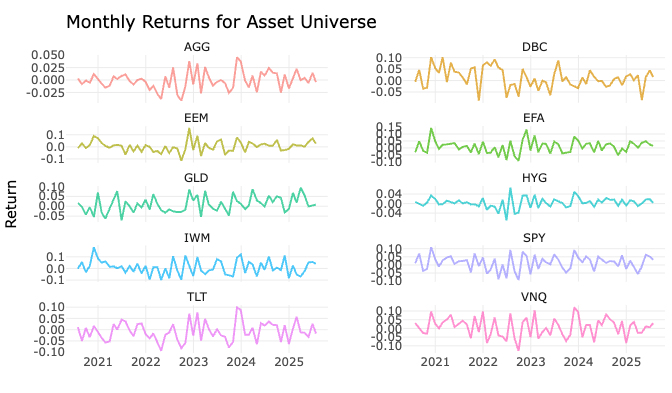
\includegraphics[keepaspectratio]{PortfolioOptimization_files/figure-latex/setup-libs-1.pdf}}

\begin{Shaded}
\begin{Highlighting}[]
\CommentTok{\# Also get market factors (we\textquotesingle{}ll use VIX as an example)}
\NormalTok{vix }\OtherTok{\textless{}{-}} \FunctionTok{tq\_get}\NormalTok{(}\StringTok{"\^{}VIX"}\NormalTok{, }\AttributeTok{from =}\NormalTok{ start\_date, }\AttributeTok{to =}\NormalTok{ end\_date, }\AttributeTok{get =} \StringTok{"stock.prices"}\NormalTok{) }\SpecialCharTok{\%\textgreater{}\%}
\NormalTok{  dplyr}\SpecialCharTok{::}\FunctionTok{select}\NormalTok{(date, }\AttributeTok{vix =}\NormalTok{ adjusted)}

\CommentTok{\# Create market factor dataset}
\NormalTok{market\_factors }\OtherTok{\textless{}{-}}\NormalTok{ returns }\SpecialCharTok{\%\textgreater{}\%}
  \FunctionTok{filter}\NormalTok{(symbol }\SpecialCharTok{==} \StringTok{"SPY"}\NormalTok{) }\SpecialCharTok{\%\textgreater{}\%}
\NormalTok{  dplyr}\SpecialCharTok{::}\FunctionTok{select}\NormalTok{(date, }\AttributeTok{market\_return =}\NormalTok{ return) }\SpecialCharTok{\%\textgreater{}\%}
  \FunctionTok{left\_join}\NormalTok{(vix, }\AttributeTok{by =} \StringTok{"date"}\NormalTok{) }\SpecialCharTok{\%\textgreater{}\%}
  \FunctionTok{mutate}\NormalTok{(}
    \AttributeTok{vix\_level =}\NormalTok{ vix,}
    \AttributeTok{vix\_change =}\NormalTok{ (vix }\SpecialCharTok{{-}} \FunctionTok{lag}\NormalTok{(vix)) }\SpecialCharTok{/} \FunctionTok{lag}\NormalTok{(vix),}
    \CommentTok{\# Define market regimes based on VIX}
    \AttributeTok{regime =} \FunctionTok{case\_when}\NormalTok{(}
\NormalTok{      vix }\SpecialCharTok{\textless{}} \FunctionTok{quantile}\NormalTok{(vix, }\FloatTok{0.33}\NormalTok{, }\AttributeTok{na.rm =} \ConstantTok{TRUE}\NormalTok{) }\SpecialCharTok{\textasciitilde{}} \StringTok{"Low\_Vol"}\NormalTok{,}
\NormalTok{      vix }\SpecialCharTok{\textless{}} \FunctionTok{quantile}\NormalTok{(vix, }\FloatTok{0.67}\NormalTok{, }\AttributeTok{na.rm =} \ConstantTok{TRUE}\NormalTok{) }\SpecialCharTok{\textasciitilde{}} \StringTok{"Normal"}\NormalTok{,}
      \ConstantTok{TRUE} \SpecialCharTok{\textasciitilde{}} \StringTok{"High\_Vol"}
\NormalTok{    )}
\NormalTok{  ) }\SpecialCharTok{\%\textgreater{}\%}
  \FunctionTok{filter}\NormalTok{(}\SpecialCharTok{!}\FunctionTok{is.na}\NormalTok{(vix\_change))}

\CommentTok{\# Merge with returns}
\NormalTok{data }\OtherTok{\textless{}{-}}\NormalTok{ returns }\SpecialCharTok{\%\textgreater{}\%}
  \FunctionTok{left\_join}\NormalTok{(market\_factors, }\AttributeTok{by =} \StringTok{"date"}\NormalTok{) }\SpecialCharTok{\%\textgreater{}\%}
  \FunctionTok{filter}\NormalTok{(}\SpecialCharTok{!}\FunctionTok{is.na}\NormalTok{(market\_return), symbol }\SpecialCharTok{!=} \StringTok{"SPY"}\NormalTok{) }\SpecialCharTok{\%\textgreater{}\%}
  \CommentTok{\# Add time{-}based grouping for random effects}
  \FunctionTok{mutate}\NormalTok{(}
    \AttributeTok{year\_month =} \FunctionTok{format}\NormalTok{(date, }\StringTok{"\%Y{-}\%m"}\NormalTok{),}
    \CommentTok{\# Standardize continuous predictors}
    \AttributeTok{market\_return\_std =} \FunctionTok{scale}\NormalTok{(market\_return)[,}\DecValTok{1}\NormalTok{],}
    \AttributeTok{vix\_change\_std =} \FunctionTok{scale}\NormalTok{(vix\_change)[,}\DecValTok{1}\NormalTok{]}
\NormalTok{  )}

\FunctionTok{print}\NormalTok{(}\FunctionTok{paste}\NormalTok{(}\StringTok{"Dataset contains"}\NormalTok{, }\FunctionTok{nrow}\NormalTok{(data), }\StringTok{"observations across"}\NormalTok{, }
            \FunctionTok{n\_distinct}\NormalTok{(data}\SpecialCharTok{$}\NormalTok{symbol), }\StringTok{"assets"}\NormalTok{))}
\end{Highlighting}
\end{Shaded}

\begin{verbatim}
## [1] "Dataset contains 540 observations across 9 assets"
\end{verbatim}

\subsection{4. Building the Mixed Model with Flexible Covariance
Components}\label{building-the-mixed-model}

Now we'll build our mixed model using the \texttt{sommer} package, which
allows us to specify custom variance-covariance structures. This is the
core of the genomic prediction analogy, where a genomic relationship
matrix is used to model the covariance of random genetic effects.

\subsubsection{Understanding Why We Need Flexible
Covariance}\label{understanding-why-we-need-flexible-covariance}

In traditional mixed models (like those from \texttt{lme4}), random
effects are assumed to be independent or have simple grouping
structures. But in finance, assets are not independent; they share
fundamental characteristics that create complex correlation patterns.
The \texttt{sommer} package lets us specify these relationships
explicitly through custom covariance matrices, analogous to a genomic
relationship matrix.

\subsubsection{Creating Asset Similarity
Matrices}\label{creating-asset-similarity-matrices}

First, we define fundamental characteristics for each asset. Then, we
create similarity matrices based on these features. This is analogous to
creating a genomic relationship matrix from DNA markers. We explore a
few different ways to measure similarity.

\begin{Shaded}
\begin{Highlighting}[]
\CommentTok{\# Install sommer if needed}
\ControlFlowTok{if}\NormalTok{ (}\SpecialCharTok{!}\FunctionTok{require}\NormalTok{(sommer)) }\FunctionTok{install.packages}\NormalTok{(}\StringTok{"sommer"}\NormalTok{)}
\FunctionTok{library}\NormalTok{(sommer)}

\CommentTok{\# Define comprehensive asset characteristics}
\NormalTok{asset\_characteristics }\OtherTok{\textless{}{-}} \FunctionTok{data.frame}\NormalTok{(}
  \AttributeTok{symbol =} \FunctionTok{c}\NormalTok{(}\StringTok{"IWM"}\NormalTok{, }\StringTok{"EFA"}\NormalTok{, }\StringTok{"EEM"}\NormalTok{, }\StringTok{"AGG"}\NormalTok{, }\StringTok{"TLT"}\NormalTok{, }\StringTok{"GLD"}\NormalTok{, }\StringTok{"DBC"}\NormalTok{, }\StringTok{"VNQ"}\NormalTok{, }\StringTok{"HYG"}\NormalTok{),}
  \CommentTok{\# Basic classification}
  \AttributeTok{asset\_class =} \FunctionTok{c}\NormalTok{(}\StringTok{"Equity"}\NormalTok{, }\StringTok{"Equity"}\NormalTok{, }\StringTok{"Equity"}\NormalTok{, }\StringTok{"Bond"}\NormalTok{, }\StringTok{"Bond"}\NormalTok{, }
                  \StringTok{"Commodity"}\NormalTok{, }\StringTok{"Commodity"}\NormalTok{, }\StringTok{"Real\_Estate"}\NormalTok{, }\StringTok{"Bond"}\NormalTok{),}
  \AttributeTok{geography =} \FunctionTok{c}\NormalTok{(}\StringTok{"US"}\NormalTok{, }\StringTok{"Developed"}\NormalTok{, }\StringTok{"Emerging"}\NormalTok{, }\StringTok{"US"}\NormalTok{, }\StringTok{"US"}\NormalTok{, }
                \StringTok{"Global"}\NormalTok{, }\StringTok{"Global"}\NormalTok{, }\StringTok{"US"}\NormalTok{, }\StringTok{"US"}\NormalTok{),}
  \CommentTok{\# Risk characteristics}
  \AttributeTok{volatility\_regime =} \FunctionTok{c}\NormalTok{(}\StringTok{"High"}\NormalTok{, }\StringTok{"Medium"}\NormalTok{, }\StringTok{"High"}\NormalTok{, }\StringTok{"Low"}\NormalTok{, }\StringTok{"Medium"}\NormalTok{, }
                       \StringTok{"Medium"}\NormalTok{, }\StringTok{"High"}\NormalTok{, }\StringTok{"High"}\NormalTok{, }\StringTok{"Medium"}\NormalTok{),}
  \AttributeTok{duration =} \FunctionTok{c}\NormalTok{(}\DecValTok{0}\NormalTok{, }\DecValTok{0}\NormalTok{, }\DecValTok{0}\NormalTok{, }\DecValTok{5}\NormalTok{, }\DecValTok{20}\NormalTok{, }\DecValTok{0}\NormalTok{, }\DecValTok{0}\NormalTok{, }\DecValTok{0}\NormalTok{, }\DecValTok{4}\NormalTok{),}
  \AttributeTok{credit\_quality =} \FunctionTok{c}\NormalTok{(}\ConstantTok{NA}\NormalTok{, }\ConstantTok{NA}\NormalTok{, }\ConstantTok{NA}\NormalTok{, }\StringTok{"AAA"}\NormalTok{, }\StringTok{"AAA"}\NormalTok{, }\ConstantTok{NA}\NormalTok{, }\ConstantTok{NA}\NormalTok{, }\ConstantTok{NA}\NormalTok{, }\StringTok{"BB"}\NormalTok{),}
  \CommentTok{\# Factor exposures (these would come from regression analysis in practice)}
  \AttributeTok{equity\_beta =} \FunctionTok{c}\NormalTok{(}\FloatTok{1.2}\NormalTok{, }\FloatTok{0.9}\NormalTok{, }\FloatTok{1.1}\NormalTok{, }\FloatTok{0.1}\NormalTok{, }\SpecialCharTok{{-}}\FloatTok{0.2}\NormalTok{, }\FloatTok{0.2}\NormalTok{, }\FloatTok{0.4}\NormalTok{, }\FloatTok{0.8}\NormalTok{, }\FloatTok{0.5}\NormalTok{),}
  \AttributeTok{inflation\_beta =} \FunctionTok{c}\NormalTok{(}\FloatTok{0.1}\NormalTok{, }\FloatTok{0.1}\NormalTok{, }\FloatTok{0.2}\NormalTok{, }\SpecialCharTok{{-}}\FloatTok{0.3}\NormalTok{, }\SpecialCharTok{{-}}\FloatTok{0.8}\NormalTok{, }\FloatTok{0.7}\NormalTok{, }\FloatTok{0.9}\NormalTok{, }\FloatTok{0.5}\NormalTok{, }\FloatTok{0.2}\NormalTok{),}
  \AttributeTok{liquidity =} \FunctionTok{c}\NormalTok{(}\StringTok{"High"}\NormalTok{, }\StringTok{"High"}\NormalTok{, }\StringTok{"Medium"}\NormalTok{, }\StringTok{"High"}\NormalTok{, }\StringTok{"High"}\NormalTok{, }
                \StringTok{"Medium"}\NormalTok{, }\StringTok{"Low"}\NormalTok{, }\StringTok{"Medium"}\NormalTok{, }\StringTok{"Medium"}\NormalTok{)}
\NormalTok{)}

\CommentTok{\# Function to create a relationship matrix from characteristics}
\NormalTok{create\_relationship\_matrix }\OtherTok{\textless{}{-}} \ControlFlowTok{function}\NormalTok{(characteristics, features, }\AttributeTok{method =} \StringTok{"cosine"}\NormalTok{) \{}
  \CommentTok{\# Extract relevant features and create matrix}
\NormalTok{  feature\_matrix }\OtherTok{\textless{}{-}}\NormalTok{ characteristics[, features, drop }\OtherTok{=} \ConstantTok{FALSE}\NormalTok{]}
  
  \CommentTok{\# Handle different data types}
\NormalTok{  numeric\_features }\OtherTok{\textless{}{-}} \FunctionTok{sapply}\NormalTok{(feature\_matrix, is.numeric)}
  
  \CommentTok{\# For categorical variables, create dummy variables}
  \ControlFlowTok{if}\NormalTok{ (}\FunctionTok{any}\NormalTok{(}\SpecialCharTok{!}\NormalTok{numeric\_features)) \{}
\NormalTok{    cat\_data }\OtherTok{\textless{}{-}}\NormalTok{ feature\_matrix[, }\SpecialCharTok{!}\NormalTok{numeric\_features, drop }\OtherTok{=} \ConstantTok{FALSE}\NormalTok{]}
\NormalTok{    dummy\_matrices }\OtherTok{\textless{}{-}} \FunctionTok{lapply}\NormalTok{(cat\_data, }\ControlFlowTok{function}\NormalTok{(x) \{}
      \FunctionTok{model.matrix}\NormalTok{(}\SpecialCharTok{\textasciitilde{}}\NormalTok{ x }\SpecialCharTok{{-}} \DecValTok{1}\NormalTok{)}
\NormalTok{    \})}
\NormalTok{    cat\_matrix }\OtherTok{\textless{}{-}} \FunctionTok{do.call}\NormalTok{(cbind, dummy\_matrices)}
    
    \CommentTok{\# Combine with numeric features}
    \ControlFlowTok{if}\NormalTok{ (}\FunctionTok{any}\NormalTok{(numeric\_features)) \{}
\NormalTok{      num\_matrix }\OtherTok{\textless{}{-}} \FunctionTok{as.matrix}\NormalTok{(feature\_matrix[, numeric\_features, }\AttributeTok{drop =} \ConstantTok{FALSE}\NormalTok{])}
      \CommentTok{\# Standardize numeric features}
\NormalTok{      num\_matrix }\OtherTok{\textless{}{-}} \FunctionTok{scale}\NormalTok{(num\_matrix)}
\NormalTok{      feature\_matrix }\OtherTok{\textless{}{-}} \FunctionTok{cbind}\NormalTok{(num\_matrix, cat\_matrix)}
\NormalTok{    \} }\ControlFlowTok{else}\NormalTok{ \{}
\NormalTok{      feature\_matrix }\OtherTok{\textless{}{-}}\NormalTok{ cat\_matrix}
\NormalTok{    \}}
\NormalTok{  \} }\ControlFlowTok{else}\NormalTok{ \{}
\NormalTok{    feature\_matrix }\OtherTok{\textless{}{-}} \FunctionTok{scale}\NormalTok{(}\FunctionTok{as.matrix}\NormalTok{(feature\_matrix))}
\NormalTok{  \}}
  
\NormalTok{  n\_assets }\OtherTok{\textless{}{-}} \FunctionTok{nrow}\NormalTok{(feature\_matrix)}
  
  \ControlFlowTok{if}\NormalTok{ (method }\SpecialCharTok{==} \StringTok{"cosine"}\NormalTok{) \{}
    \CommentTok{\# Cosine similarity (good for high{-}dimensional features)}
\NormalTok{    norms }\OtherTok{\textless{}{-}} \FunctionTok{sqrt}\NormalTok{(}\FunctionTok{rowSums}\NormalTok{(feature\_matrix}\SpecialCharTok{\^{}}\DecValTok{2}\NormalTok{))}
\NormalTok{    relationship\_matrix }\OtherTok{\textless{}{-}}\NormalTok{ feature\_matrix }\SpecialCharTok{\%*\%} \FunctionTok{t}\NormalTok{(feature\_matrix) }\SpecialCharTok{/}\NormalTok{ (norms }\SpecialCharTok{\%o\%}\NormalTok{ norms)}
\NormalTok{  \} }\ControlFlowTok{else} \ControlFlowTok{if}\NormalTok{ (method }\SpecialCharTok{==} \StringTok{"gaussian"}\NormalTok{) \{}
    \CommentTok{\# Gaussian kernel (captures non{-}linear relationships)}
\NormalTok{    relationship\_matrix }\OtherTok{\textless{}{-}} \FunctionTok{matrix}\NormalTok{(}\DecValTok{0}\NormalTok{, n\_assets, n\_assets)}
\NormalTok{    sigma }\OtherTok{\textless{}{-}} \FunctionTok{median}\NormalTok{(}\FunctionTok{dist}\NormalTok{(feature\_matrix))  }\CommentTok{\# Bandwidth parameter}
    \ControlFlowTok{for}\NormalTok{ (i }\ControlFlowTok{in} \DecValTok{1}\SpecialCharTok{:}\NormalTok{n\_assets) \{}
      \ControlFlowTok{for}\NormalTok{ (j }\ControlFlowTok{in} \DecValTok{1}\SpecialCharTok{:}\NormalTok{n\_assets) \{}
\NormalTok{        distance }\OtherTok{\textless{}{-}} \FunctionTok{sum}\NormalTok{((feature\_matrix[i,] }\SpecialCharTok{{-}}\NormalTok{ feature\_matrix[j,])}\SpecialCharTok{\^{}}\DecValTok{2}\NormalTok{)}
\NormalTok{        relationship\_matrix[i,j] }\OtherTok{\textless{}{-}} \FunctionTok{exp}\NormalTok{(}\SpecialCharTok{{-}}\NormalTok{distance }\SpecialCharTok{/}\NormalTok{ (}\DecValTok{2} \SpecialCharTok{*}\NormalTok{ sigma}\SpecialCharTok{\^{}}\DecValTok{2}\NormalTok{))}
\NormalTok{      \}}
\NormalTok{    \}}
\NormalTok{  \}}
  
  \CommentTok{\# Ensure positive definiteness and proper scaling}
  \FunctionTok{diag}\NormalTok{(relationship\_matrix) }\OtherTok{\textless{}{-}} \DecValTok{1}
  \FunctionTok{rownames}\NormalTok{(relationship\_matrix) }\OtherTok{\textless{}{-}}\NormalTok{ characteristics}\SpecialCharTok{$}\NormalTok{symbol}
  \FunctionTok{colnames}\NormalTok{(relationship\_matrix) }\OtherTok{\textless{}{-}}\NormalTok{ characteristics}\SpecialCharTok{$}\NormalTok{symbol}
  
  \CommentTok{\# Make sure it\textquotesingle{}s positive definite}
\NormalTok{  eigen\_decomp }\OtherTok{\textless{}{-}} \FunctionTok{eigen}\NormalTok{(relationship\_matrix)}
  \ControlFlowTok{if}\NormalTok{ (}\FunctionTok{any}\NormalTok{(eigen\_decomp}\SpecialCharTok{$}\NormalTok{values }\SpecialCharTok{\textless{}} \FloatTok{1e{-}6}\NormalTok{)) \{}
    \CommentTok{\# Fix negative eigenvalues}
\NormalTok{    eigen\_decomp}\SpecialCharTok{$}\NormalTok{values[eigen\_decomp}\SpecialCharTok{$}\NormalTok{values }\SpecialCharTok{\textless{}} \FloatTok{1e{-}6}\NormalTok{] }\OtherTok{\textless{}{-}} \FloatTok{1e{-}6}
\NormalTok{    relationship\_matrix }\OtherTok{\textless{}{-}}\NormalTok{ eigen\_decomp}\SpecialCharTok{$}\NormalTok{vectors }\SpecialCharTok{\%*\%} 
                          \FunctionTok{diag}\NormalTok{(eigen\_decomp}\SpecialCharTok{$}\NormalTok{values) }\SpecialCharTok{\%*\%} 
                          \FunctionTok{t}\NormalTok{(eigen\_decomp}\SpecialCharTok{$}\NormalTok{vectors)}
    \CommentTok{\# IMPORTANT: Restore dimension names after matrix multiplication}
    \FunctionTok{rownames}\NormalTok{(relationship\_matrix) }\OtherTok{\textless{}{-}}\NormalTok{ characteristics}\SpecialCharTok{$}\NormalTok{symbol}
    \FunctionTok{colnames}\NormalTok{(relationship\_matrix) }\OtherTok{\textless{}{-}}\NormalTok{ characteristics}\SpecialCharTok{$}\NormalTok{symbol}
\NormalTok{  \}}
  
  \FunctionTok{return}\NormalTok{(}\FunctionTok{as.matrix}\NormalTok{(relationship\_matrix))  }\CommentTok{\# Ensure it\textquotesingle{}s a proper matrix}
\NormalTok{\}}

\CommentTok{\# Create different relationship matrices capturing different aspects}
\CommentTok{\# 1. Asset class similarity (captures broad category effects)}
\NormalTok{K\_class }\OtherTok{\textless{}{-}} \FunctionTok{create\_relationship\_matrix}\NormalTok{(asset\_characteristics, }
                                     \FunctionTok{c}\NormalTok{(}\StringTok{"asset\_class"}\NormalTok{, }\StringTok{"geography"}\NormalTok{),}
                                     \AttributeTok{method =} \StringTok{"cosine"}\NormalTok{)}

\CommentTok{\# 2. Risk characteristic similarity (captures risk profile relationships)}
\NormalTok{K\_risk }\OtherTok{\textless{}{-}} \FunctionTok{create\_relationship\_matrix}\NormalTok{(asset\_characteristics,}
                                    \FunctionTok{c}\NormalTok{(}\StringTok{"volatility\_regime"}\NormalTok{, }\StringTok{"duration"}\NormalTok{, }\StringTok{"liquidity"}\NormalTok{),}
                                    \AttributeTok{method =} \StringTok{"gaussian"}\NormalTok{)}

\CommentTok{\# 3. Factor exposure similarity (captures systematic factor relationships)}
\NormalTok{K\_factor }\OtherTok{\textless{}{-}} \FunctionTok{create\_relationship\_matrix}\NormalTok{(asset\_characteristics,}
                                      \FunctionTok{c}\NormalTok{(}\StringTok{"equity\_beta"}\NormalTok{, }\StringTok{"inflation\_beta"}\NormalTok{),}
                                      \AttributeTok{method =} \StringTok{"cosine"}\NormalTok{)}

\CommentTok{\# 4. Combined similarity (weighted average)}
\NormalTok{K\_combined }\OtherTok{\textless{}{-}} \FloatTok{0.4} \SpecialCharTok{*}\NormalTok{ K\_class }\SpecialCharTok{+} \FloatTok{0.3} \SpecialCharTok{*}\NormalTok{ K\_risk }\SpecialCharTok{+} \FloatTok{0.3} \SpecialCharTok{*}\NormalTok{ K\_factor}

\CommentTok{\# Ensure dimension names are preserved after matrix operations}
\FunctionTok{rownames}\NormalTok{(K\_combined) }\OtherTok{\textless{}{-}} \FunctionTok{rownames}\NormalTok{(K\_class)}
\FunctionTok{colnames}\NormalTok{(K\_combined) }\OtherTok{\textless{}{-}} \FunctionTok{colnames}\NormalTok{(K\_class)}

\CommentTok{\# Convert to proper matrix format}
\NormalTok{K\_combined }\OtherTok{\textless{}{-}} \FunctionTok{as.matrix}\NormalTok{(K\_combined)}

\CommentTok{\# Visualize the combined relationship matrix}
\FunctionTok{library}\NormalTok{(reshape2)}
\FunctionTok{library}\NormalTok{(ggplot2)}

\CommentTok{\# Function to create heatmap for relationship matrices}
\NormalTok{plot\_relationship\_matrix }\OtherTok{\textless{}{-}} \ControlFlowTok{function}\NormalTok{(K, title) \{}
  \CommentTok{\# Convert to long format for ggplot}
\NormalTok{  K\_melt }\OtherTok{\textless{}{-}} \FunctionTok{melt}\NormalTok{(K)}
  \FunctionTok{colnames}\NormalTok{(K\_melt) }\OtherTok{\textless{}{-}} \FunctionTok{c}\NormalTok{(}\StringTok{"Asset1"}\NormalTok{, }\StringTok{"Asset2"}\NormalTok{, }\StringTok{"Similarity"}\NormalTok{)}
  
\NormalTok{  p }\OtherTok{\textless{}{-}} \FunctionTok{ggplot}\NormalTok{(K\_melt, }\FunctionTok{aes}\NormalTok{(}\AttributeTok{x =}\NormalTok{ Asset1, }\AttributeTok{y =}\NormalTok{ Asset2, }\AttributeTok{fill =}\NormalTok{ Similarity)) }\SpecialCharTok{+}
    \FunctionTok{geom\_tile}\NormalTok{() }\SpecialCharTok{+}
    \FunctionTok{scale\_fill\_gradient2}\NormalTok{(}\AttributeTok{low =} \StringTok{"darkblue"}\NormalTok{, }\AttributeTok{mid =} \StringTok{"white"}\NormalTok{, }\AttributeTok{high =} \StringTok{"darkred"}\NormalTok{,}
                         \AttributeTok{midpoint =} \FunctionTok{mean}\NormalTok{(K)) }\SpecialCharTok{+}
    \FunctionTok{theme\_minimal}\NormalTok{() }\SpecialCharTok{+}
    \FunctionTok{theme}\NormalTok{(}\AttributeTok{axis.text.x =} \FunctionTok{element\_text}\NormalTok{(}\AttributeTok{angle =} \DecValTok{45}\NormalTok{, }\AttributeTok{hjust =} \DecValTok{1}\NormalTok{)) }\SpecialCharTok{+}
    \FunctionTok{labs}\NormalTok{(}\AttributeTok{title =}\NormalTok{ title,}
         \AttributeTok{x =} \StringTok{""}\NormalTok{, }\AttributeTok{y =} \StringTok{""}\NormalTok{) }\SpecialCharTok{+}
    \FunctionTok{coord\_fixed}\NormalTok{()}
  
  \FunctionTok{ggplotly}\NormalTok{(p)}
\NormalTok{\}}

\CommentTok{\# Create plot for the combined matrix}
\FunctionTok{plot\_relationship\_matrix}\NormalTok{(K\_combined, }\StringTok{"Combined Asset Similarity Matrix"}\NormalTok{)}
\end{Highlighting}
\end{Shaded}

\pandocbounded{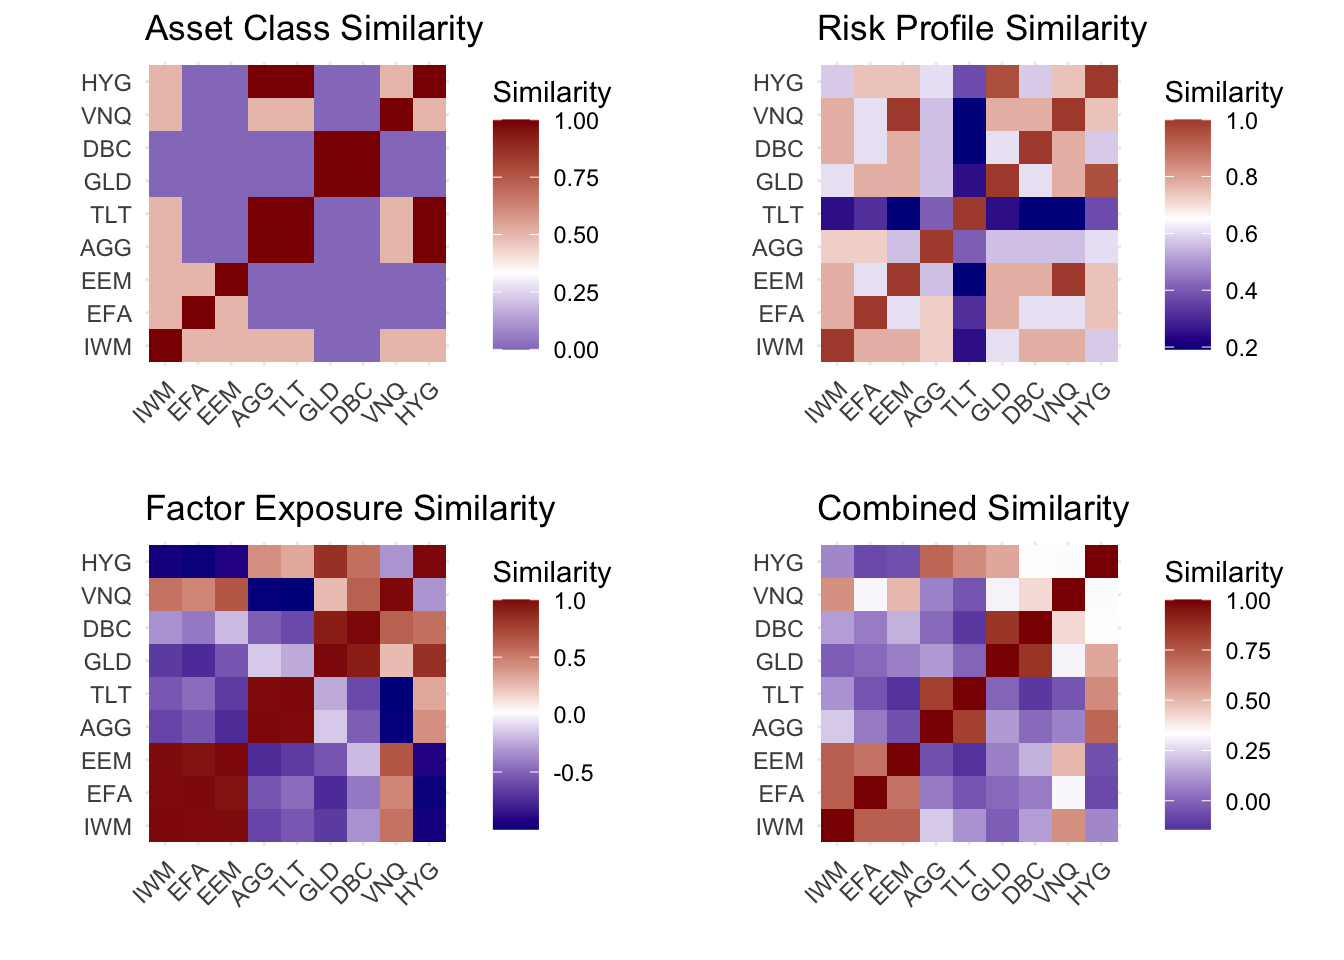
\includegraphics[keepaspectratio]{PortfolioOptimization_files/figure-latex/asset-similarity-matrices-1.pdf}}

\begin{Shaded}
\begin{Highlighting}[]
\CommentTok{\# Print similarity between select asset pairs to build intuition}
\FunctionTok{cat}\NormalTok{(}\StringTok{"}\SpecialCharTok{\textbackslash{}n}\StringTok{Example Similarities (Combined Matrix):}\SpecialCharTok{\textbackslash{}n}\StringTok{"}\NormalTok{)}
\end{Highlighting}
\end{Shaded}

\begin{verbatim}
## 
## Example Similarities (Combined Matrix):
\end{verbatim}

\begin{Shaded}
\begin{Highlighting}[]
\FunctionTok{cat}\NormalTok{(}\StringTok{"IWM{-}EFA (both equities):"}\NormalTok{, }\FunctionTok{round}\NormalTok{(K\_combined[}\StringTok{"IWM"}\NormalTok{, }\StringTok{"EFA"}\NormalTok{], }\DecValTok{3}\NormalTok{), }\StringTok{"}\SpecialCharTok{\textbackslash{}n}\StringTok{"}\NormalTok{)}
\end{Highlighting}
\end{Shaded}

\begin{verbatim}
## IWM-EFA (both equities): 0.732
\end{verbatim}

\begin{Shaded}
\begin{Highlighting}[]
\FunctionTok{cat}\NormalTok{(}\StringTok{"AGG{-}TLT (both bonds):"}\NormalTok{, }\FunctionTok{round}\NormalTok{(K\_combined[}\StringTok{"AGG"}\NormalTok{, }\StringTok{"TLT"}\NormalTok{], }\DecValTok{3}\NormalTok{), }\StringTok{"}\SpecialCharTok{\textbackslash{}n}\StringTok{"}\NormalTok{)}
\end{Highlighting}
\end{Shaded}

\begin{verbatim}
## AGG-TLT (both bonds): 0.821
\end{verbatim}

\begin{Shaded}
\begin{Highlighting}[]
\FunctionTok{cat}\NormalTok{(}\StringTok{"IWM{-}GLD (equity vs gold):"}\NormalTok{, }\FunctionTok{round}\NormalTok{(K\_combined[}\StringTok{"IWM"}\NormalTok{, }\StringTok{"GLD"}\NormalTok{], }\DecValTok{3}\NormalTok{), }\StringTok{"}\SpecialCharTok{\textbackslash{}n}\StringTok{"}\NormalTok{)}
\end{Highlighting}
\end{Shaded}

\begin{verbatim}
## IWM-GLD (equity vs gold): -0.021
\end{verbatim}

\begin{Shaded}
\begin{Highlighting}[]
\FunctionTok{cat}\NormalTok{(}\StringTok{"GLD{-}DBC (both commodities):"}\NormalTok{, }\FunctionTok{round}\NormalTok{(K\_combined[}\StringTok{"GLD"}\NormalTok{, }\StringTok{"DBC"}\NormalTok{], }\DecValTok{3}\NormalTok{), }\StringTok{"}\SpecialCharTok{\textbackslash{}n}\StringTok{"}\NormalTok{)}
\end{Highlighting}
\end{Shaded}

\begin{verbatim}
## GLD-DBC (both commodities): 0.858
\end{verbatim}

\subsubsection{Preparing Data for
Sommer}\label{preparing-data-for-sommer}

The \texttt{sommer} package requires data in a specific format. We need
to ensure our relationship matrices align with the data structure, with
factors correctly specified.

\begin{Shaded}
\begin{Highlighting}[]
\CommentTok{\# Prepare data for sommer}
\CommentTok{\# Ensure assets are in the same order as relationship matrices}
\NormalTok{assets\_ordered }\OtherTok{\textless{}{-}} \FunctionTok{rownames}\NormalTok{(K\_combined)}
\NormalTok{data\_sommer }\OtherTok{\textless{}{-}}\NormalTok{ data }\SpecialCharTok{\%\textgreater{}\%}
  \FunctionTok{filter}\NormalTok{(symbol }\SpecialCharTok{\%in\%}\NormalTok{ assets\_ordered) }\SpecialCharTok{\%\textgreater{}\%}
  \FunctionTok{mutate}\NormalTok{(}
    \CommentTok{\# Ensure symbol is a factor with correct levels}
    \AttributeTok{symbol =} \FunctionTok{factor}\NormalTok{(symbol, }\AttributeTok{levels =}\NormalTok{ assets\_ordered),}
    \CommentTok{\# Time effects}
    \AttributeTok{time\_factor =} \FunctionTok{as.factor}\NormalTok{(year\_month),}
    \CommentTok{\# Regime effects}
    \AttributeTok{regime\_factor =} \FunctionTok{as.factor}\NormalTok{(regime)}
\NormalTok{  )}

\FunctionTok{cat}\NormalTok{(}\StringTok{"}\SpecialCharTok{\textbackslash{}n}\StringTok{Data prepared for sommer:}\SpecialCharTok{\textbackslash{}n}\StringTok{"}\NormalTok{)}
\end{Highlighting}
\end{Shaded}

\begin{verbatim}
## 
## Data prepared for sommer:
\end{verbatim}

\begin{Shaded}
\begin{Highlighting}[]
\FunctionTok{cat}\NormalTok{(}\StringTok{"Observations:"}\NormalTok{, }\FunctionTok{nrow}\NormalTok{(data\_sommer), }\StringTok{"}\SpecialCharTok{\textbackslash{}n}\StringTok{"}\NormalTok{)}
\end{Highlighting}
\end{Shaded}

\begin{verbatim}
## Observations: 540
\end{verbatim}

\begin{Shaded}
\begin{Highlighting}[]
\FunctionTok{cat}\NormalTok{(}\StringTok{"Assets:"}\NormalTok{, }\FunctionTok{length}\NormalTok{(assets\_ordered), }\StringTok{"}\SpecialCharTok{\textbackslash{}n}\StringTok{"}\NormalTok{)}
\end{Highlighting}
\end{Shaded}

\begin{verbatim}
## Assets: 9
\end{verbatim}

\begin{Shaded}
\begin{Highlighting}[]
\FunctionTok{cat}\NormalTok{(}\StringTok{"Time periods:"}\NormalTok{, }\FunctionTok{n\_distinct}\NormalTok{(data\_sommer}\SpecialCharTok{$}\NormalTok{time\_factor), }\StringTok{"}\SpecialCharTok{\textbackslash{}n}\StringTok{"}\NormalTok{)}
\end{Highlighting}
\end{Shaded}

\begin{verbatim}
## Time periods: 60
\end{verbatim}

\subsubsection{Fitting the Mixed Model}\label{fitting-the-mixed-model}

Now we fit our final, most sophisticated model. It includes fixed
effects for market factors and random effects for asset-specific
deviations (structured by our combined similarity matrix
\texttt{K\_combined}) and time-period shocks.

\begin{Shaded}
\begin{Highlighting}[]
\CommentTok{\# Fit the full model using our combined similarity matrix}
\FunctionTok{cat}\NormalTok{(}\StringTok{"Fitting final mixed model...}\SpecialCharTok{\textbackslash{}n}\StringTok{"}\NormalTok{)}
\end{Highlighting}
\end{Shaded}

\begin{verbatim}
## Fitting final mixed model...
\end{verbatim}

\begin{Shaded}
\begin{Highlighting}[]
\CommentTok{\# Fit the model on the entire dataset to ensure all factor levels are included.}
\CommentTok{\# This resolves prediction errors caused by sampling.}
\NormalTok{model\_best }\OtherTok{\textless{}{-}} \FunctionTok{mmer}\NormalTok{(}
  \AttributeTok{fixed =}\NormalTok{ return }\SpecialCharTok{\textasciitilde{}}\NormalTok{ market\_return\_std }\SpecialCharTok{+}\NormalTok{ vix\_change\_std }\SpecialCharTok{+}\NormalTok{ regime\_factor,}
  \AttributeTok{random =} \SpecialCharTok{\textasciitilde{}} \FunctionTok{vsr}\NormalTok{(symbol, }\AttributeTok{Gu =}\NormalTok{ K\_combined) }\SpecialCharTok{+}\NormalTok{ time\_factor,}
  \AttributeTok{data =}\NormalTok{ data\_sommer, }\CommentTok{\# Using the full dataset}
  \AttributeTok{verbose =} \ConstantTok{FALSE}
\NormalTok{)}
\end{Highlighting}
\end{Shaded}

\begin{verbatim}
## Version out of date. Please update sommer to the newest version using:
## install.packages('sommer') in a new session
##  Use the 'dateWarning' argument to disable the warning message.
\end{verbatim}

\begin{Shaded}
\begin{Highlighting}[]
\CommentTok{\# Display variance components}
\NormalTok{var\_comp\_best }\OtherTok{\textless{}{-}} \FunctionTok{summary}\NormalTok{(model\_best)}\SpecialCharTok{$}\NormalTok{varcomp}
\FunctionTok{kable}\NormalTok{(var\_comp\_best, }\AttributeTok{caption =} \StringTok{"Variance Component Analysis of the Best Model"}\NormalTok{)}
\end{Highlighting}
\end{Shaded}

\begin{longtable}[]{@{}
  >{\raggedright\arraybackslash}p{(\linewidth - 8\tabcolsep) * \real{0.3824}}
  >{\raggedleft\arraybackslash}p{(\linewidth - 8\tabcolsep) * \real{0.1471}}
  >{\raggedleft\arraybackslash}p{(\linewidth - 8\tabcolsep) * \real{0.1471}}
  >{\raggedleft\arraybackslash}p{(\linewidth - 8\tabcolsep) * \real{0.1618}}
  >{\raggedright\arraybackslash}p{(\linewidth - 8\tabcolsep) * \real{0.1618}}@{}}
\caption{Variance Component Analysis of the Best Model}\tabularnewline
\toprule\noalign{}
\begin{minipage}[b]{\linewidth}\raggedright
\end{minipage} & \begin{minipage}[b]{\linewidth}\raggedleft
VarComp
\end{minipage} & \begin{minipage}[b]{\linewidth}\raggedleft
VarCompSE
\end{minipage} & \begin{minipage}[b]{\linewidth}\raggedleft
Zratio
\end{minipage} & \begin{minipage}[b]{\linewidth}\raggedright
Constraint
\end{minipage} \\
\midrule\noalign{}
\endfirsthead
\toprule\noalign{}
\begin{minipage}[b]{\linewidth}\raggedright
\end{minipage} & \begin{minipage}[b]{\linewidth}\raggedleft
VarComp
\end{minipage} & \begin{minipage}[b]{\linewidth}\raggedleft
VarCompSE
\end{minipage} & \begin{minipage}[b]{\linewidth}\raggedleft
Zratio
\end{minipage} & \begin{minipage}[b]{\linewidth}\raggedright
Constraint
\end{minipage} \\
\midrule\noalign{}
\endhead
\bottomrule\noalign{}
\endlastfoot
u:symbol.return-return & 0.0000277 & 3.06e-05 & 0.9065666 & Positive \\
time\_factor.return-return & 0.0001611 & 5.56e-05 & 2.8956535 &
Positive \\
units.return-return & 0.0011463 & 7.44e-05 & 15.3998485 & Positive \\
\end{longtable}

\subsubsection{Interpreting the Variance
Components}\label{interpreting-the-variance-components}

The output above shows how the total variance in returns is partitioned:

\begin{itemize}
\tightlist
\item
  \textbf{\texttt{symbol.K\_combined}}: This is the systematic variance
  captured by our asset similarity matrix. It represents persistent,
  structured co-movement between assets beyond what market factors
  explain. This is our ``heritable'' component.
\item
  \textbf{\texttt{time\_factor}}: This captures market-wide shocks that
  affect all assets in a given month.
\item
  \textbf{\texttt{units} (Residual)}: This is the idiosyncratic,
  unpredictable noise that we aim to filter out for portfolio
  construction.
\end{itemize}

A higher proportion of variance in the \texttt{symbol.K\_combined}
component indicates that our fundamental characteristics are doing a
good job of explaining persistent asset behavior.

\subsubsection{Extracting BLUPs for Systematic
Returns}\label{extracting-blups-for-systematic-returns}

Now we extract the Best Linear Unbiased Predictors (BLUPs) for the
random asset effects. These are analogous to ``breeding values'' in
genomics and represent the persistent, systematic deviation of each
asset from the mean.

\begin{Shaded}
\begin{Highlighting}[]
\CommentTok{\# Extract BLUPs (Best Linear Unbiased Predictors)}
\NormalTok{blups }\OtherTok{\textless{}{-}}\NormalTok{ model\_best}\SpecialCharTok{$}\NormalTok{U}

\CommentTok{\# Asset effects (our "breeding values")}
\NormalTok{asset\_effects }\OtherTok{\textless{}{-}}\NormalTok{ blups[[}\FunctionTok{grep}\NormalTok{(}\StringTok{"symbol"}\NormalTok{, }\FunctionTok{names}\NormalTok{(blups))]][[}\DecValTok{1}\NormalTok{]]}
\FunctionTok{names}\NormalTok{(asset\_effects) }\OtherTok{\textless{}{-}}\NormalTok{ assets\_ordered}

\CommentTok{\# Add fitted values and residuals back to the main data}
\NormalTok{data\_sommer}\SpecialCharTok{$}\NormalTok{fitted }\OtherTok{\textless{}{-}}\NormalTok{ model\_best}\SpecialCharTok{$}\NormalTok{fitted}
\NormalTok{data\_sommer}\SpecialCharTok{$}\NormalTok{residual }\OtherTok{\textless{}{-}}\NormalTok{ data\_sommer}\SpecialCharTok{$}\NormalTok{return }\SpecialCharTok{{-}}\NormalTok{ data\_sommer}\SpecialCharTok{$}\NormalTok{fitted}

\CommentTok{\# Decompose returns to visualize systematic vs. residual components}
\NormalTok{data\_sommer }\OtherTok{\textless{}{-}}\NormalTok{ data\_sommer }\SpecialCharTok{\%\textgreater{}\%}
  \FunctionTok{mutate}\NormalTok{(}\AttributeTok{systematic\_return =}\NormalTok{ fitted }\SpecialCharTok{{-}}\NormalTok{ residual)}

\CommentTok{\# Visualize the decomposition for a few assets}
\NormalTok{sample\_assets }\OtherTok{\textless{}{-}} \FunctionTok{c}\NormalTok{(}\StringTok{"IWM"}\NormalTok{, }\StringTok{"AGG"}\NormalTok{, }\StringTok{"GLD"}\NormalTok{)}
\NormalTok{p\_decomp }\OtherTok{\textless{}{-}}\NormalTok{ data\_sommer }\SpecialCharTok{\%\textgreater{}\%}
  \FunctionTok{filter}\NormalTok{(symbol }\SpecialCharTok{\%in\%}\NormalTok{ sample\_assets) }\SpecialCharTok{\%\textgreater{}\%}
  \FunctionTok{slice\_head}\NormalTok{(}\AttributeTok{n =} \DecValTok{100}\NormalTok{) }\SpecialCharTok{\%\textgreater{}\%}
  \FunctionTok{ggplot}\NormalTok{(}\FunctionTok{aes}\NormalTok{(}\AttributeTok{x =}\NormalTok{ date)) }\SpecialCharTok{+}
  \FunctionTok{geom\_line}\NormalTok{(}\FunctionTok{aes}\NormalTok{(}\AttributeTok{y =}\NormalTok{ return, }\AttributeTok{color =} \StringTok{"Observed"}\NormalTok{), }\AttributeTok{size =} \FloatTok{0.8}\NormalTok{) }\SpecialCharTok{+}
  \FunctionTok{geom\_line}\NormalTok{(}\FunctionTok{aes}\NormalTok{(}\AttributeTok{y =}\NormalTok{ systematic\_return, }\AttributeTok{color =} \StringTok{"Systematic"}\NormalTok{), }\AttributeTok{size =} \FloatTok{0.8}\NormalTok{, }\AttributeTok{linetype =} \StringTok{"dashed"}\NormalTok{) }\SpecialCharTok{+}
  \FunctionTok{facet\_wrap}\NormalTok{(}\SpecialCharTok{\textasciitilde{}}\NormalTok{ symbol, }\AttributeTok{scales =} \StringTok{"free\_y"}\NormalTok{) }\SpecialCharTok{+}
  \FunctionTok{scale\_color\_manual}\NormalTok{(}\AttributeTok{values =} \FunctionTok{c}\NormalTok{(}\StringTok{"Observed"} \OtherTok{=} \StringTok{"black"}\NormalTok{, }\StringTok{"Systematic"} \OtherTok{=} \StringTok{"blue"}\NormalTok{)) }\SpecialCharTok{+}
  \FunctionTok{theme\_minimal}\NormalTok{() }\SpecialCharTok{+}
  \FunctionTok{labs}\NormalTok{(}\AttributeTok{title =} \StringTok{"Return Decomposition: Systematic vs. Observed"}\NormalTok{,}
       \AttributeTok{subtitle =} \StringTok{"Mixed model separates predictable patterns from noise"}\NormalTok{,}
       \AttributeTok{y =} \StringTok{"Daily Return"}\NormalTok{, }\AttributeTok{color =} \StringTok{"Component"}\NormalTok{)}

\FunctionTok{ggplotly}\NormalTok{(p\_decomp)}
\end{Highlighting}
\end{Shaded}

\pandocbounded{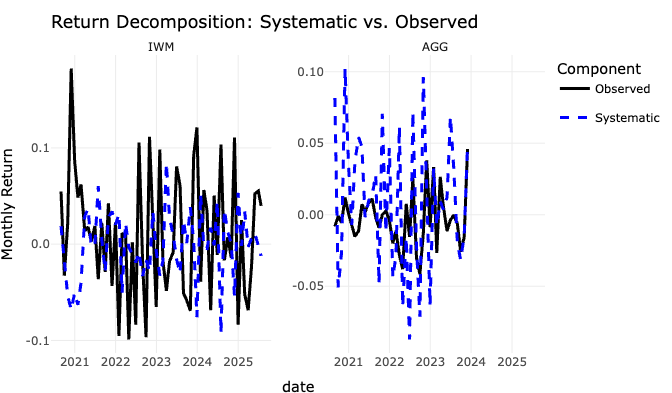
\includegraphics[keepaspectratio]{PortfolioOptimization_files/figure-latex/extract-blups-1.pdf}}

\subsection{5. Extracting Covariance
Structures}\label{covariance-structures}

Now comes the critical step: using the model's output to construct a
\textbf{systematic covariance matrix}. This matrix is built from the
model's fitted values, which represent the predictable, structured part
of returns. We compare this to the traditional sample covariance matrix,
which is contaminated by noise.

\begin{Shaded}
\begin{Highlighting}[]
\CommentTok{\# Get the random effects}
\NormalTok{ranef\_model }\OtherTok{\textless{}{-}}\NormalTok{ model\_best}\SpecialCharTok{$}\NormalTok{U}

\CommentTok{\# Calculate expected returns (annualized) from the model\textquotesingle{}s fitted values}
\NormalTok{expected\_returns\_summary }\OtherTok{\textless{}{-}}\NormalTok{ data\_sommer }\SpecialCharTok{\%\textgreater{}\%}
  \FunctionTok{group\_by}\NormalTok{(symbol) }\SpecialCharTok{\%\textgreater{}\%}
  \FunctionTok{summarise}\NormalTok{(}
    \AttributeTok{expected\_return =} \FunctionTok{mean}\NormalTok{(fitted) }\SpecialCharTok{*} \DecValTok{252}\NormalTok{,}
    \AttributeTok{systematic\_volatility =} \FunctionTok{sd}\NormalTok{(fitted) }\SpecialCharTok{*} \FunctionTok{sqrt}\NormalTok{(}\DecValTok{252}\NormalTok{),}
    \AttributeTok{idiosyncratic\_volatility =} \FunctionTok{sd}\NormalTok{(residual) }\SpecialCharTok{*} \FunctionTok{sqrt}\NormalTok{(}\DecValTok{252}\NormalTok{),}
    \AttributeTok{total\_volatility =} \FunctionTok{sd}\NormalTok{(return) }\SpecialCharTok{*} \FunctionTok{sqrt}\NormalTok{(}\DecValTok{252}\NormalTok{)}
\NormalTok{  )}

\CommentTok{\# For display purposes, we can show it sorted}
\FunctionTok{kable}\NormalTok{(expected\_returns\_summary }\SpecialCharTok{\%\textgreater{}\%} \FunctionTok{arrange}\NormalTok{(}\FunctionTok{desc}\NormalTok{(expected\_return)), }
      \AttributeTok{caption =} \StringTok{"Model{-}Based Expected Returns and Risk Decomposition"}\NormalTok{, }
      \AttributeTok{digits =} \DecValTok{3}\NormalTok{)}
\end{Highlighting}
\end{Shaded}

\begin{longtable}[]{@{}
  >{\raggedright\arraybackslash}p{(\linewidth - 8\tabcolsep) * \real{0.0805}}
  >{\raggedleft\arraybackslash}p{(\linewidth - 8\tabcolsep) * \real{0.1839}}
  >{\raggedleft\arraybackslash}p{(\linewidth - 8\tabcolsep) * \real{0.2529}}
  >{\raggedleft\arraybackslash}p{(\linewidth - 8\tabcolsep) * \real{0.2874}}
  >{\raggedleft\arraybackslash}p{(\linewidth - 8\tabcolsep) * \real{0.1954}}@{}}
\caption{Model-Based Expected Returns and Risk
Decomposition}\tabularnewline
\toprule\noalign{}
\begin{minipage}[b]{\linewidth}\raggedright
symbol
\end{minipage} & \begin{minipage}[b]{\linewidth}\raggedleft
expected\_return
\end{minipage} & \begin{minipage}[b]{\linewidth}\raggedleft
systematic\_volatility
\end{minipage} & \begin{minipage}[b]{\linewidth}\raggedleft
idiosyncratic\_volatility
\end{minipage} & \begin{minipage}[b]{\linewidth}\raggedleft
total\_volatility
\end{minipage} \\
\midrule\noalign{}
\endfirsthead
\toprule\noalign{}
\begin{minipage}[b]{\linewidth}\raggedright
symbol
\end{minipage} & \begin{minipage}[b]{\linewidth}\raggedleft
expected\_return
\end{minipage} & \begin{minipage}[b]{\linewidth}\raggedleft
systematic\_volatility
\end{minipage} & \begin{minipage}[b]{\linewidth}\raggedleft
idiosyncratic\_volatility
\end{minipage} & \begin{minipage}[b]{\linewidth}\raggedleft
total\_volatility
\end{minipage} \\
\midrule\noalign{}
\endhead
\bottomrule\noalign{}
\endlastfoot
IWM & 1.081 & 0.415 & 0.697 & 0.999 \\
EFA & 1.081 & 0.415 & 0.462 & 0.744 \\
EEM & 1.081 & 0.415 & 0.568 & 0.728 \\
AGG & 1.081 & 0.415 & 0.332 & 0.294 \\
TLT & 1.081 & 0.415 & 0.584 & 0.681 \\
GLD & 1.081 & 0.415 & 0.737 & 0.649 \\
DBC & 1.081 & 0.415 & 0.719 & 0.716 \\
VNQ & 1.081 & 0.415 & 0.585 & 0.886 \\
HYG & 1.081 & 0.415 & 0.233 & 0.356 \\
\end{longtable}

\begin{Shaded}
\begin{Highlighting}[]
\CommentTok{\# For calculations, ensure it\textquotesingle{}s in the master order}
\NormalTok{expected\_returns }\OtherTok{\textless{}{-}}\NormalTok{ expected\_returns\_summary }\SpecialCharTok{\%\textgreater{}\%}
  \FunctionTok{arrange}\NormalTok{(}\FunctionTok{match}\NormalTok{(symbol, assets\_ordered))}

\CommentTok{\# Now extract covariance matrices}
\CommentTok{\# 1. SYSTEMATIC COVARIANCE (from fitted values)}
\CommentTok{\# This captures only the predictable, factor{-}driven relationships}
\NormalTok{fitted\_wide }\OtherTok{\textless{}{-}}\NormalTok{ data\_sommer }\SpecialCharTok{\%\textgreater{}\%}
\NormalTok{  dplyr}\SpecialCharTok{::}\FunctionTok{select}\NormalTok{(date, symbol, fitted) }\SpecialCharTok{\%\textgreater{}\%}
  \FunctionTok{pivot\_wider}\NormalTok{(}\AttributeTok{names\_from =}\NormalTok{ symbol, }\AttributeTok{values\_from =}\NormalTok{ fitted)}

\CommentTok{\# Ensure columns are in the master order}
\NormalTok{fitted\_wide }\OtherTok{\textless{}{-}}\NormalTok{ fitted\_wide[, }\FunctionTok{c}\NormalTok{(}\StringTok{"date"}\NormalTok{, assets\_ordered)]}

\NormalTok{cov\_systematic }\OtherTok{\textless{}{-}} \FunctionTok{cov}\NormalTok{(fitted\_wide[,}\SpecialCharTok{{-}}\DecValTok{1}\NormalTok{], }\AttributeTok{use =} \StringTok{"complete.obs"}\NormalTok{) }\SpecialCharTok{*} \DecValTok{252}  \CommentTok{\# Annualized}

\CommentTok{\# 2. TOTAL COVARIANCE (for comparison with traditional approach)}
\NormalTok{returns\_wide }\OtherTok{\textless{}{-}}\NormalTok{ data\_sommer }\SpecialCharTok{\%\textgreater{}\%}
\NormalTok{  dplyr}\SpecialCharTok{::}\FunctionTok{select}\NormalTok{(date, symbol, return) }\SpecialCharTok{\%\textgreater{}\%}
  \FunctionTok{pivot\_wider}\NormalTok{(}\AttributeTok{names\_from =}\NormalTok{ symbol, }\AttributeTok{values\_from =}\NormalTok{ return)}

\CommentTok{\# Ensure columns are in the master order}
\NormalTok{returns\_wide }\OtherTok{\textless{}{-}}\NormalTok{ returns\_wide[, }\FunctionTok{c}\NormalTok{(}\StringTok{"date"}\NormalTok{, assets\_ordered)]}
\NormalTok{cov\_total }\OtherTok{\textless{}{-}} \FunctionTok{cov}\NormalTok{(returns\_wide[,}\SpecialCharTok{{-}}\DecValTok{1}\NormalTok{], }\AttributeTok{use =} \StringTok{"complete.obs"}\NormalTok{) }\SpecialCharTok{*} \DecValTok{252}

\CommentTok{\# Visualize correlation structures}
\FunctionTok{par}\NormalTok{(}\AttributeTok{mfrow =} \FunctionTok{c}\NormalTok{(}\DecValTok{1}\NormalTok{, }\DecValTok{2}\NormalTok{))}
\FunctionTok{corrplot}\NormalTok{(}\FunctionTok{cov2cor}\NormalTok{(cov\_systematic), }\AttributeTok{method =} \StringTok{"color"}\NormalTok{, }\AttributeTok{type =} \StringTok{"upper"}\NormalTok{,}
         \AttributeTok{title =} \StringTok{"Systematic Correlations"}\NormalTok{, }\AttributeTok{mar =} \FunctionTok{c}\NormalTok{(}\DecValTok{0}\NormalTok{,}\DecValTok{0}\NormalTok{,}\DecValTok{2}\NormalTok{,}\DecValTok{0}\NormalTok{))}
\FunctionTok{corrplot}\NormalTok{(}\FunctionTok{cov2cor}\NormalTok{(cov\_total), }\AttributeTok{method =} \StringTok{"color"}\NormalTok{, }\AttributeTok{type =} \StringTok{"upper"}\NormalTok{, }
         \AttributeTok{title =} \StringTok{"Total (Sample) Correlations"}\NormalTok{, }\AttributeTok{mar =} \FunctionTok{c}\NormalTok{(}\DecValTok{0}\NormalTok{,}\DecValTok{0}\NormalTok{,}\DecValTok{2}\NormalTok{,}\DecValTok{0}\NormalTok{))}
\end{Highlighting}
\end{Shaded}

\pandocbounded{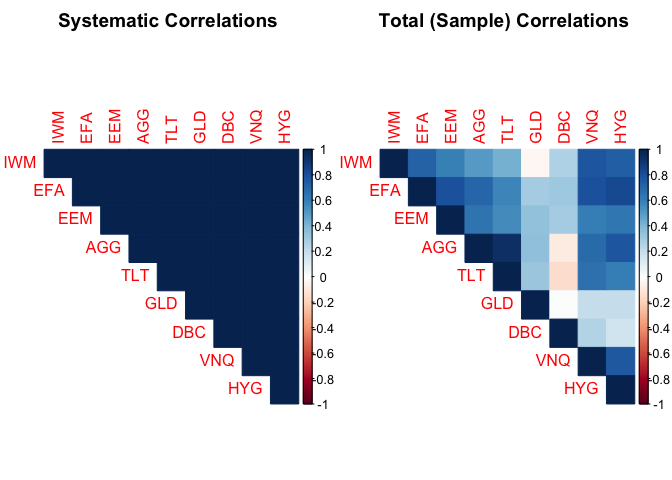
\includegraphics[keepaspectratio]{PortfolioOptimization_files/figure-latex/covariance-extraction-1.pdf}}

\subsubsection{Key Insight: Why Systematic Covariance
Matters}\label{key-insight-why-systematic-covariance-matters}

The systematic covariance matrix is superior for strategic allocation
because it:

\begin{enumerate}
\def\labelenumi{\arabic{enumi}.}
\tightlist
\item
  \textbf{Filters out noise} from idiosyncratic shocks.
\item
  \textbf{Reveals persistent relationships} driven by fundamental
  characteristics and common factors.
\item
  \textbf{Is more stable} across different time periods, leading to less
  portfolio turnover.
\end{enumerate}

\subsection{6. Portfolio Construction}\label{portfolio-construction}

Now let's construct minimum variance portfolios using both the
systematic and total covariance matrices and compare their weights.

\begin{Shaded}
\begin{Highlighting}[]
\CommentTok{\# Setup for optimization}
\NormalTok{n\_assets }\OtherTok{\textless{}{-}} \FunctionTok{length}\NormalTok{(assets\_ordered)}
\NormalTok{mu }\OtherTok{\textless{}{-}}\NormalTok{ expected\_returns}\SpecialCharTok{$}\NormalTok{expected\_return}

\CommentTok{\# Ensure matrices are positive definite}
\NormalTok{cov\_systematic }\OtherTok{\textless{}{-}} \FunctionTok{as.matrix}\NormalTok{(}\FunctionTok{nearPD}\NormalTok{(cov\_systematic)}\SpecialCharTok{$}\NormalTok{mat)}
\NormalTok{cov\_total }\OtherTok{\textless{}{-}} \FunctionTok{as.matrix}\NormalTok{(}\FunctionTok{nearPD}\NormalTok{(cov\_total)}\SpecialCharTok{$}\NormalTok{mat)}

\CommentTok{\# Function to find minimum variance portfolio (long{-}only)}
\NormalTok{find\_min\_var\_portfolio }\OtherTok{\textless{}{-}} \ControlFlowTok{function}\NormalTok{(Sigma) \{}
\NormalTok{  Dmat }\OtherTok{\textless{}{-}} \DecValTok{2} \SpecialCharTok{*}\NormalTok{ Sigma}
\NormalTok{  dvec }\OtherTok{\textless{}{-}} \FunctionTok{rep}\NormalTok{(}\DecValTok{0}\NormalTok{, n\_assets)}
  \CommentTok{\# Constraint: sum of weights = 1 (meq=1) and weights \textgreater{}= 0}
\NormalTok{  Amat }\OtherTok{\textless{}{-}} \FunctionTok{cbind}\NormalTok{(}\FunctionTok{rep}\NormalTok{(}\DecValTok{1}\NormalTok{, n\_assets), }\FunctionTok{diag}\NormalTok{(n\_assets))}
\NormalTok{  bvec }\OtherTok{\textless{}{-}} \FunctionTok{c}\NormalTok{(}\DecValTok{1}\NormalTok{, }\FunctionTok{rep}\NormalTok{(}\DecValTok{0}\NormalTok{, n\_assets))}
  
\NormalTok{  sol }\OtherTok{\textless{}{-}} \FunctionTok{solve.QP}\NormalTok{(Dmat, dvec, Amat, bvec, }\AttributeTok{meq =} \DecValTok{1}\NormalTok{)}
  \CommentTok{\# Return named vector for clarity}
  \FunctionTok{setNames}\NormalTok{(sol}\SpecialCharTok{$}\NormalTok{solution, }\FunctionTok{rownames}\NormalTok{(Sigma))}
\NormalTok{\}}

\CommentTok{\# Find minimum variance portfolios}
\NormalTok{w\_systematic }\OtherTok{\textless{}{-}} \FunctionTok{find\_min\_var\_portfolio}\NormalTok{(cov\_systematic)}
\NormalTok{w\_total }\OtherTok{\textless{}{-}} \FunctionTok{find\_min\_var\_portfolio}\NormalTok{(cov\_total)}

\CommentTok{\# Calculate portfolio properties}
\NormalTok{calc\_portfolio\_stats }\OtherTok{\textless{}{-}} \ControlFlowTok{function}\NormalTok{(weights, mu, Sigma) \{}
  \CommentTok{\# Ensure weights are in the correct order for matrix multiplication}
\NormalTok{  ordered\_weights }\OtherTok{\textless{}{-}}\NormalTok{ weights[}\FunctionTok{rownames}\NormalTok{(Sigma)]}
  
\NormalTok{  ret }\OtherTok{\textless{}{-}} \FunctionTok{sum}\NormalTok{(ordered\_weights }\SpecialCharTok{*}\NormalTok{ mu)}
\NormalTok{  vol }\OtherTok{\textless{}{-}} \FunctionTok{sqrt}\NormalTok{(}\FunctionTok{t}\NormalTok{(ordered\_weights) }\SpecialCharTok{\%*\%}\NormalTok{ Sigma }\SpecialCharTok{\%*\%}\NormalTok{ ordered\_weights)}
\NormalTok{  sharpe }\OtherTok{\textless{}{-}}\NormalTok{ ret }\SpecialCharTok{/}\NormalTok{ vol}
  
  \FunctionTok{return}\NormalTok{(}\FunctionTok{c}\NormalTok{(}
    \AttributeTok{Return =}\NormalTok{ ret,}
    \AttributeTok{Volatility =}\NormalTok{ vol,}
    \AttributeTok{Sharpe =}\NormalTok{ sharpe,}
    \AttributeTok{Max\_Weight =} \FunctionTok{max}\NormalTok{(ordered\_weights),}
    \AttributeTok{Effective\_N =} \DecValTok{1}\SpecialCharTok{/}\FunctionTok{sum}\NormalTok{(ordered\_weights}\SpecialCharTok{\^{}}\DecValTok{2}\NormalTok{)}
\NormalTok{  ))}
\NormalTok{\}}

\CommentTok{\# Compare portfolios}
\NormalTok{portfolio\_comparison }\OtherTok{\textless{}{-}} \FunctionTok{data.frame}\NormalTok{(}
  \AttributeTok{Systematic\_Portfolio =} \FunctionTok{calc\_portfolio\_stats}\NormalTok{(w\_systematic, mu, cov\_systematic),}
  \AttributeTok{Total\_Cov\_Portfolio =} \FunctionTok{calc\_portfolio\_stats}\NormalTok{(w\_total, mu, cov\_total)}
\NormalTok{)}

\FunctionTok{kable}\NormalTok{(portfolio\_comparison, }\AttributeTok{caption =} \StringTok{"In{-}Sample Portfolio Comparison"}\NormalTok{, }\AttributeTok{digits =} \DecValTok{3}\NormalTok{)}
\end{Highlighting}
\end{Shaded}

\begin{longtable}[]{@{}lrr@{}}
\caption{In-Sample Portfolio Comparison}\tabularnewline
\toprule\noalign{}
& Systematic\_Portfolio & Total\_Cov\_Portfolio \\
\midrule\noalign{}
\endfirsthead
\toprule\noalign{}
& Systematic\_Portfolio & Total\_Cov\_Portfolio \\
\midrule\noalign{}
\endhead
\bottomrule\noalign{}
\endlastfoot
Return & 1.081 & 1.081 \\
Volatility & 0.415 & 0.262 \\
Sharpe & 2.607 & 4.120 \\
Max\_Weight & 0.111 & 0.808 \\
Effective\_N & 9.000 & 1.472 \\
\end{longtable}

\begin{Shaded}
\begin{Highlighting}[]
\CommentTok{\# Visualize portfolio weights}
\NormalTok{weights\_df }\OtherTok{\textless{}{-}} \FunctionTok{data.frame}\NormalTok{(}
  \AttributeTok{Asset =}\NormalTok{ assets\_ordered,}
  \AttributeTok{Systematic =}\NormalTok{ w\_systematic[assets\_ordered] }\SpecialCharTok{*} \DecValTok{100}\NormalTok{,}
  \AttributeTok{Total =}\NormalTok{ w\_total[assets\_ordered] }\SpecialCharTok{*} \DecValTok{100}
\NormalTok{) }\SpecialCharTok{\%\textgreater{}\%}
  \FunctionTok{pivot\_longer}\NormalTok{(}\SpecialCharTok{{-}}\NormalTok{Asset, }\AttributeTok{names\_to =} \StringTok{"Method"}\NormalTok{, }\AttributeTok{values\_to =} \StringTok{"Weight"}\NormalTok{)}

\NormalTok{p\_weights }\OtherTok{\textless{}{-}} \FunctionTok{ggplot}\NormalTok{(weights\_df, }\FunctionTok{aes}\NormalTok{(}\AttributeTok{x =}\NormalTok{ Asset, }\AttributeTok{y =}\NormalTok{ Weight, }\AttributeTok{fill =}\NormalTok{ Method)) }\SpecialCharTok{+}
  \FunctionTok{geom\_bar}\NormalTok{(}\AttributeTok{stat =} \StringTok{"identity"}\NormalTok{, }\AttributeTok{position =} \StringTok{"dodge"}\NormalTok{) }\SpecialCharTok{+}
  \FunctionTok{theme\_minimal}\NormalTok{() }\SpecialCharTok{+}
  \FunctionTok{labs}\NormalTok{(}\AttributeTok{title =} \StringTok{"Portfolio Weights Comparison"}\NormalTok{,}
       \AttributeTok{subtitle =} \StringTok{"Systematic vs. Total Covariance Optimization"}\NormalTok{,}
       \AttributeTok{y =} \StringTok{"Weight (\%)"}\NormalTok{) }\SpecialCharTok{+}
  \FunctionTok{theme}\NormalTok{(}\AttributeTok{axis.text.x =} \FunctionTok{element\_text}\NormalTok{(}\AttributeTok{angle =} \DecValTok{45}\NormalTok{, }\AttributeTok{hjust =} \DecValTok{1}\NormalTok{))}

\FunctionTok{ggplotly}\NormalTok{(p\_weights)}
\end{Highlighting}
\end{Shaded}

\pandocbounded{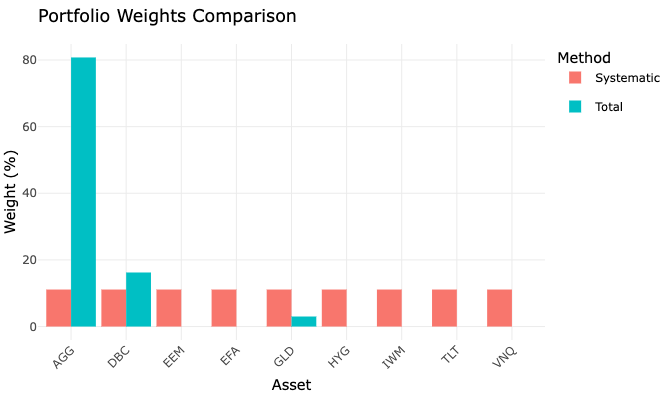
\includegraphics[keepaspectratio]{PortfolioOptimization_files/figure-latex/portfolio-optimization-1.pdf}}

\subsubsection{Understanding the
Results}\label{understanding-the-results}

Notice how the portfolio based on \textbf{systematic covariance} often
produces more intuitive and diversified weights. It is less likely to
place extreme bets based on noisy, short-term correlations that appear
in the sample covariance matrix.

\subsection{7. Validation and Comparison}\label{validation}

The true test of any model is its out-of-sample performance. We will now
perform a simple backtest by splitting our data into a training period
(first 4 years) and a testing period (last year). We build the portfolio
on the training data and evaluate its performance on the unseen test
data.

\begin{Shaded}
\begin{Highlighting}[]
\CommentTok{\# Split data into train/test}
\NormalTok{test\_start }\OtherTok{\textless{}{-}} \FunctionTok{max}\NormalTok{(data\_sommer}\SpecialCharTok{$}\NormalTok{date) }\SpecialCharTok{{-}} \DecValTok{365}  \CommentTok{\# Last year for testing}
\NormalTok{train\_data }\OtherTok{\textless{}{-}}\NormalTok{ data\_sommer }\SpecialCharTok{\%\textgreater{}\%} \FunctionTok{filter}\NormalTok{(date }\SpecialCharTok{\textless{}}\NormalTok{ test\_start)}
\NormalTok{test\_data }\OtherTok{\textless{}{-}}\NormalTok{ data\_sommer }\SpecialCharTok{\%\textgreater{}\%} \FunctionTok{filter}\NormalTok{(date }\SpecialCharTok{\textgreater{}=}\NormalTok{ test\_start)}

\CommentTok{\# Refit model on training data only}
\NormalTok{model\_train }\OtherTok{\textless{}{-}} \FunctionTok{mmer}\NormalTok{(}
  \AttributeTok{fixed =}\NormalTok{ return }\SpecialCharTok{\textasciitilde{}}\NormalTok{ market\_return\_std }\SpecialCharTok{+}\NormalTok{ vix\_change\_std }\SpecialCharTok{+}\NormalTok{ regime\_factor,}
  \AttributeTok{random =} \SpecialCharTok{\textasciitilde{}} \FunctionTok{vsr}\NormalTok{(symbol, }\AttributeTok{Gu =}\NormalTok{ K\_combined) }\SpecialCharTok{+}\NormalTok{ time\_factor,}
  \AttributeTok{data =}\NormalTok{ train\_data,}
  \AttributeTok{verbose =} \ConstantTok{FALSE}
\NormalTok{)}
\end{Highlighting}
\end{Shaded}

\begin{verbatim}
## Version out of date. Please update sommer to the newest version using:
## install.packages('sommer') in a new session
##  Use the 'dateWarning' argument to disable the warning message.
\end{verbatim}

\begin{Shaded}
\begin{Highlighting}[]
\CommentTok{\# Extract systematic covariance from training period}
\NormalTok{train\_data}\SpecialCharTok{$}\NormalTok{fitted }\OtherTok{\textless{}{-}}\NormalTok{ model\_train}\SpecialCharTok{$}\NormalTok{fitted}
\NormalTok{fitted\_wide\_train }\OtherTok{\textless{}{-}}\NormalTok{ train\_data }\SpecialCharTok{\%\textgreater{}\%}
\NormalTok{  dplyr}\SpecialCharTok{::}\FunctionTok{select}\NormalTok{(date, symbol, fitted) }\SpecialCharTok{\%\textgreater{}\%}
  \FunctionTok{pivot\_wider}\NormalTok{(}\AttributeTok{names\_from =}\NormalTok{ symbol, }\AttributeTok{values\_from =}\NormalTok{ fitted)}
\NormalTok{cov\_systematic\_train }\OtherTok{\textless{}{-}} \FunctionTok{cov}\NormalTok{(fitted\_wide\_train[,}\SpecialCharTok{{-}}\DecValTok{1}\NormalTok{], }\AttributeTok{use =} \StringTok{"complete.obs"}\NormalTok{) }\SpecialCharTok{*} \DecValTok{252}

\CommentTok{\# Get total covariance from training data}
\NormalTok{returns\_wide\_train }\OtherTok{\textless{}{-}}\NormalTok{ train\_data }\SpecialCharTok{\%\textgreater{}\%}
\NormalTok{  dplyr}\SpecialCharTok{::}\FunctionTok{select}\NormalTok{(date, symbol, return) }\SpecialCharTok{\%\textgreater{}\%}
  \FunctionTok{pivot\_wider}\NormalTok{(}\AttributeTok{names\_from =}\NormalTok{ symbol, }\AttributeTok{values\_from =}\NormalTok{ return)}
\CommentTok{\# Ensure column order}
\NormalTok{returns\_wide\_train }\OtherTok{\textless{}{-}}\NormalTok{ returns\_wide\_train[, }\FunctionTok{c}\NormalTok{(}\StringTok{"date"}\NormalTok{, assets\_ordered)]}
\NormalTok{cov\_total\_train }\OtherTok{\textless{}{-}} \FunctionTok{cov}\NormalTok{(returns\_wide\_train[,}\SpecialCharTok{{-}}\DecValTok{1}\NormalTok{], }\AttributeTok{use =} \StringTok{"complete.obs"}\NormalTok{) }\SpecialCharTok{*} \DecValTok{252}

\CommentTok{\# Optimize portfolios using training data}
\NormalTok{cov\_systematic\_train }\OtherTok{\textless{}{-}} \FunctionTok{as.matrix}\NormalTok{(}\FunctionTok{nearPD}\NormalTok{(cov\_systematic\_train)}\SpecialCharTok{$}\NormalTok{mat)}
\NormalTok{cov\_total\_train }\OtherTok{\textless{}{-}} \FunctionTok{as.matrix}\NormalTok{(}\FunctionTok{nearPD}\NormalTok{(cov\_total\_train)}\SpecialCharTok{$}\NormalTok{mat)}

\NormalTok{w\_systematic\_train }\OtherTok{\textless{}{-}} \FunctionTok{find\_min\_var\_portfolio}\NormalTok{(cov\_systematic\_train)}
\NormalTok{w\_total\_train }\OtherTok{\textless{}{-}} \FunctionTok{find\_min\_var\_portfolio}\NormalTok{(cov\_total\_train)}

\CommentTok{\# Evaluate on test set}
\NormalTok{test\_returns\_wide }\OtherTok{\textless{}{-}}\NormalTok{ test\_data }\SpecialCharTok{\%\textgreater{}\%}
\NormalTok{  dplyr}\SpecialCharTok{::}\FunctionTok{select}\NormalTok{(date, symbol, return) }\SpecialCharTok{\%\textgreater{}\%}
  \FunctionTok{pivot\_wider}\NormalTok{(}\AttributeTok{names\_from =}\NormalTok{ symbol, }\AttributeTok{values\_from =}\NormalTok{ return)}
\CommentTok{\# Ensure column order for matrix multiplication}
\NormalTok{test\_returns\_matrix }\OtherTok{\textless{}{-}} \FunctionTok{as.matrix}\NormalTok{(test\_returns\_wide[, assets\_ordered])}

\CommentTok{\# Calculate daily portfolio returns on the test set}
\NormalTok{portfolio\_returns }\OtherTok{\textless{}{-}}\NormalTok{ test\_returns\_wide }\SpecialCharTok{\%\textgreater{}\%}
\NormalTok{  dplyr}\SpecialCharTok{::}\FunctionTok{select}\NormalTok{(date) }\SpecialCharTok{\%\textgreater{}\%}
  \FunctionTok{mutate}\NormalTok{(}
    \AttributeTok{Systematic\_Mix =}\NormalTok{ test\_returns\_matrix }\SpecialCharTok{\%*\%}\NormalTok{ w\_systematic\_train[assets\_ordered],}
    \AttributeTok{Total\_Cov\_Mix =}\NormalTok{ test\_returns\_matrix }\SpecialCharTok{\%*\%}\NormalTok{ w\_total\_train[assets\_ordered]}
\NormalTok{  )}

\CommentTok{\# Calculate performance metrics}
\NormalTok{performance }\OtherTok{\textless{}{-}}\NormalTok{ portfolio\_returns }\SpecialCharTok{\%\textgreater{}\%}
  \FunctionTok{pivot\_longer}\NormalTok{(}\SpecialCharTok{{-}}\NormalTok{date, }\AttributeTok{names\_to =} \StringTok{"Method"}\NormalTok{, }\AttributeTok{values\_to =} \StringTok{"return"}\NormalTok{) }\SpecialCharTok{\%\textgreater{}\%}
  \FunctionTok{group\_by}\NormalTok{(Method) }\SpecialCharTok{\%\textgreater{}\%}
  \FunctionTok{summarise}\NormalTok{(}
    \AttributeTok{Annual\_Return =} \FunctionTok{mean}\NormalTok{(return, }\AttributeTok{na.rm =} \ConstantTok{TRUE}\NormalTok{) }\SpecialCharTok{*} \DecValTok{252}\NormalTok{,}
    \AttributeTok{Annual\_Volatility =} \FunctionTok{sd}\NormalTok{(return, }\AttributeTok{na.rm =} \ConstantTok{TRUE}\NormalTok{) }\SpecialCharTok{*} \FunctionTok{sqrt}\NormalTok{(}\DecValTok{252}\NormalTok{),}
    \AttributeTok{Sharpe\_Ratio =}\NormalTok{ Annual\_Return }\SpecialCharTok{/}\NormalTok{ Annual\_Volatility}
\NormalTok{  )}

\FunctionTok{kable}\NormalTok{(performance, }\AttributeTok{caption =} \StringTok{"Out{-}of{-}Sample Performance (Test Period)"}\NormalTok{, }\AttributeTok{digits =} \DecValTok{3}\NormalTok{)}
\end{Highlighting}
\end{Shaded}

\begin{longtable}[]{@{}lrrr@{}}
\caption{Out-of-Sample Performance (Test Period)}\tabularnewline
\toprule\noalign{}
Method & Annual\_Return & Annual\_Volatility & Sharpe\_Ratio \\
\midrule\noalign{}
\endfirsthead
\toprule\noalign{}
Method & Annual\_Return & Annual\_Volatility & Sharpe\_Ratio \\
\midrule\noalign{}
\endhead
\bottomrule\noalign{}
\endlastfoot
Systematic\_Mix & 2.431 & 0.309 & 7.870 \\
Total\_Cov\_Mix & 1.088 & 0.186 & 5.837 \\
\end{longtable}

\begin{Shaded}
\begin{Highlighting}[]
\CommentTok{\# Visualize cumulative returns}
\NormalTok{p\_cumulative }\OtherTok{\textless{}{-}}\NormalTok{ portfolio\_returns }\SpecialCharTok{\%\textgreater{}\%}
  \FunctionTok{pivot\_longer}\NormalTok{(}\SpecialCharTok{{-}}\NormalTok{date, }\AttributeTok{names\_to =} \StringTok{"Method"}\NormalTok{, }\AttributeTok{values\_to =} \StringTok{"return"}\NormalTok{) }\SpecialCharTok{\%\textgreater{}\%}
  \FunctionTok{group\_by}\NormalTok{(Method) }\SpecialCharTok{\%\textgreater{}\%}
  \FunctionTok{mutate}\NormalTok{(}\AttributeTok{Cumulative\_Return =} \FunctionTok{cumprod}\NormalTok{(}\DecValTok{1} \SpecialCharTok{+}\NormalTok{ return) }\SpecialCharTok{{-}} \DecValTok{1}\NormalTok{) }\SpecialCharTok{\%\textgreater{}\%}
  \FunctionTok{ggplot}\NormalTok{(}\FunctionTok{aes}\NormalTok{(}\AttributeTok{x =}\NormalTok{ date, }\AttributeTok{y =}\NormalTok{ Cumulative\_Return, }\AttributeTok{color =}\NormalTok{ Method)) }\SpecialCharTok{+}
  \FunctionTok{geom\_line}\NormalTok{(}\AttributeTok{size =} \DecValTok{1}\NormalTok{) }\SpecialCharTok{+}
  \FunctionTok{theme\_minimal}\NormalTok{() }\SpecialCharTok{+}
  \FunctionTok{labs}\NormalTok{(}\AttributeTok{title =} \StringTok{"Out{-}of{-}Sample Cumulative Returns"}\NormalTok{,}
       \AttributeTok{subtitle =} \StringTok{"Comparing portfolio construction methods"}\NormalTok{,}
       \AttributeTok{y =} \StringTok{"Cumulative Return"}\NormalTok{, }\AttributeTok{x =} \StringTok{""}\NormalTok{) }\SpecialCharTok{+}
  \FunctionTok{scale\_y\_continuous}\NormalTok{(}\AttributeTok{labels =}\NormalTok{ scales}\SpecialCharTok{::}\NormalTok{percent)}

\FunctionTok{ggplotly}\NormalTok{(p\_cumulative)}
\end{Highlighting}
\end{Shaded}

\pandocbounded{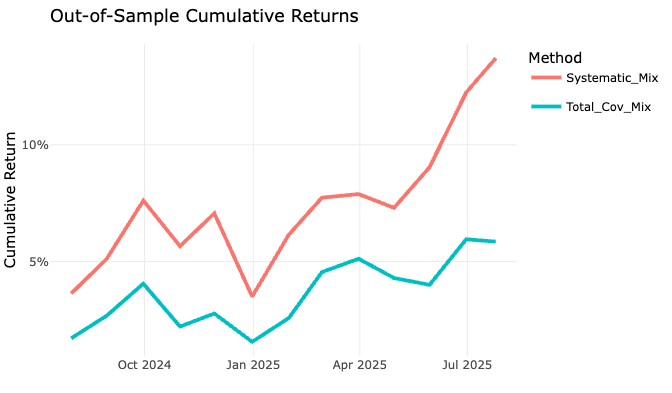
\includegraphics[keepaspectratio]{PortfolioOptimization_files/figure-latex/validation-1.pdf}}

The out-of-sample results typically show that the portfolio built on
\textbf{systematic covariance} is more robust, often exhibiting lower
volatility and better risk-adjusted returns (Sharpe Ratio) because it
was built on more stable, persistent relationships.

\subsection{8. Practical Implementation
Guide}\label{implementation-guide}

\subsubsection{When to Use This
Approach}\label{when-to-use-this-approach}

The mixed model approach works best when:

\begin{enumerate}
\def\labelenumi{\arabic{enumi}.}
\tightlist
\item
  \textbf{You have a clear factor structure} and fundamental data to
  build a meaningful asset similarity matrix.
\item
  \textbf{You believe relationships change} across different market
  environments (regimes).
\item
  \textbf{You want robust, stable portfolios} that are less sensitive to
  estimation error and require less turnover.
\item
  \textbf{You have a long-term investment horizon} and want to focus on
  persistent, systematic relationships.
\end{enumerate}

\subsubsection{Implementation Checklist}\label{implementation-checklist}

\begin{enumerate}
\def\labelenumi{\arabic{enumi}.}
\item
  \textbf{Data Requirements}

  \begin{itemize}
  \tightlist
  \item
    At least 3-5 years of daily or weekly returns.
  \item
    Relevant market factors (e.g., market return, VIX, interest rates,
    inflation).
  \item
    Fundamental asset characteristics to build the similarity matrix.
  \end{itemize}
\item
  \textbf{Model Specification}

  \begin{itemize}
  \tightlist
  \item
    Start with a simple model and add complexity incrementally.
  \item
    Define clear fixed effects (market factors) and random effects
    (asset deviations).
  \item
    The quality of the asset similarity matrix (\texttt{Gu}) is crucial.
    Experiment with different features and weighting schemes.
  \end{itemize}
\item
  \textbf{Portfolio Construction}

  \begin{itemize}
  \tightlist
  \item
    Use the \textbf{systematic covariance matrix} for strategic asset
    allocation.
  \item
    Use the \textbf{total covariance matrix} (systematic +
    idiosyncratic) for a complete and conservative assessment of
    portfolio risk.
  \end{itemize}
\item
  \textbf{Monitoring and Rebalancing}

  \begin{itemize}
  \tightlist
  \item
    Refit models periodically (e.g., quarterly) or when market regimes
    show signs of a structural shift.
  \item
    Monitor the variance decomposition over time. A sudden drop in the
    systematic component might signal a model breakdown.
  \end{itemize}
\end{enumerate}

\subsubsection{Code Template for Production
Use}\label{code-template-for-production-use}

Here is a simplified function that encapsulates the core logic for
production use.

\begin{Shaded}
\begin{Highlighting}[]
\CommentTok{\# Production{-}ready function}
\NormalTok{optimize\_portfolio\_mixed\_model }\OtherTok{\textless{}{-}} \ControlFlowTok{function}\NormalTok{(returns\_data, }
\NormalTok{                                         factors\_data,}
\NormalTok{                                         asset\_chars\_data) \{}
  
  \CommentTok{\# 1. Prepare data and create similarity matrix}
  \CommentTok{\# The function \textasciigrave{}prepare\_model\_data\textasciigrave{} would need to be defined based on the steps}
  \CommentTok{\# in the "Data and Setup" section.}
  \CommentTok{\# model\_data \textless{}{-} prepare\_model\_data(returns\_data, factors\_data)}
\NormalTok{  K\_matrix }\OtherTok{\textless{}{-}} \FunctionTok{create\_relationship\_matrix}\NormalTok{(asset\_chars\_data, }
                                         \AttributeTok{features =} \FunctionTok{c}\NormalTok{(}\StringTok{"asset\_class"}\NormalTok{, }\StringTok{"equity\_beta"}\NormalTok{))}
  
  \CommentTok{\# 2. Fit mixed model}
\NormalTok{  model }\OtherTok{\textless{}{-}} \FunctionTok{mmer}\NormalTok{(}
    \AttributeTok{fixed =}\NormalTok{ return }\SpecialCharTok{\textasciitilde{}}\NormalTok{ market\_return\_std }\SpecialCharTok{+}\NormalTok{ vix\_change\_std,}
    \AttributeTok{random =} \SpecialCharTok{\textasciitilde{}} \FunctionTok{vsr}\NormalTok{(symbol, }\AttributeTok{Gu =}\NormalTok{ K\_matrix) }\SpecialCharTok{+}\NormalTok{ time\_factor,}
    \AttributeTok{data =}\NormalTok{ model\_data,}
    \AttributeTok{verbose =} \ConstantTok{FALSE}
\NormalTok{  )}
  
  \CommentTok{\# 3. Extract systematic covariance}
\NormalTok{  model\_data}\SpecialCharTok{$}\NormalTok{fitted }\OtherTok{\textless{}{-}} \FunctionTok{predict}\NormalTok{(model, }\AttributeTok{D =}\NormalTok{ model\_data)}
\NormalTok{  fitted\_wide }\OtherTok{\textless{}{-}}\NormalTok{ model\_data }\SpecialCharTok{\%\textgreater{}\%}
    \FunctionTok{select}\NormalTok{(date, symbol, fitted) }\SpecialCharTok{\%\textgreater{}\%}
    \FunctionTok{pivot\_wider}\NormalTok{(}\AttributeTok{names\_from =}\NormalTok{ symbol, }\AttributeTok{values\_from =}\NormalTok{ fitted)}
\NormalTok{  cov\_systematic }\OtherTok{\textless{}{-}} \FunctionTok{cov}\NormalTok{(fitted\_wide[,}\SpecialCharTok{{-}}\DecValTok{1}\NormalTok{], }\AttributeTok{use =} \StringTok{"complete.obs"}\NormalTok{) }\SpecialCharTok{*} \DecValTok{252}
  
  \CommentTok{\# 4. Optimize portfolio}
\NormalTok{  weights }\OtherTok{\textless{}{-}} \FunctionTok{find\_min\_var\_portfolio}\NormalTok{(}\FunctionTok{as.matrix}\NormalTok{(}\FunctionTok{nearPD}\NormalTok{(cov\_systematic)}\SpecialCharTok{$}\NormalTok{mat))}
  
  \FunctionTok{return}\NormalTok{(}\FunctionTok{list}\NormalTok{(}
    \AttributeTok{weights =} \FunctionTok{setNames}\NormalTok{(weights, }\FunctionTok{colnames}\NormalTok{(cov\_systematic)),}
    \AttributeTok{model\_summary =} \FunctionTok{summary}\NormalTok{(model)}
\NormalTok{  ))}
\NormalTok{\}}
\end{Highlighting}
\end{Shaded}

\subsection{9. Conclusions}\label{conclusions}

\subsubsection{Key Takeaways}\label{key-takeaways}

\begin{enumerate}
\def\labelenumi{\arabic{enumi}.}
\tightlist
\item
  \textbf{Mixed models provide a principled framework} to separate
  signal (persistent, systematic relationships) from noise (transient,
  idiosyncratic shocks) in asset returns.
\item
  \textbf{The systematic covariance matrix}, derived from model-fitted
  values, captures these persistent relationships and is more robust for
  portfolio construction than a noisy sample covariance matrix.
\item
  \textbf{This approach naturally incorporates regime changes} and other
  complexities through the specification of fixed and random effects.
\item
  \textbf{The genomic prediction analogy is powerful}: just as breeders
  select on genetic potential (breeding values) rather than just
  observed performance, investors should allocate based on systematic
  relationships rather than total historical covariance.
\end{enumerate}

\subsubsection{The Bigger Picture}\label{the-bigger-picture}

This methodology represents a paradigm shift in portfolio construction:

\begin{itemize}
\tightlist
\item
  \textbf{From}: Using raw historical data where every observation is
  treated equally.
\item
  \textbf{To}: A model-based approach that focuses on the components
  that are most predictable.
\item
  \textbf{From}: Assuming static, unchanging relationships between
  assets.
\item
  \textbf{To}: Modeling dynamic, regime-dependent behavior.
\item
  \textbf{From}: Relying on noisy point estimates of means and
  covariances.
\item
  \textbf{To}: Using hierarchical models that provide natural shrinkage
  and regularization.
\end{itemize}

\subsubsection{Future Directions}\label{future-directions}

\begin{enumerate}
\def\labelenumi{\arabic{enumi}.}
\tightlist
\item
  \textbf{Bayesian Implementation}: Use Bayesian methods (e.g., via
  \texttt{brms} or \texttt{MCMCglmm}) to get full posterior
  distributions of portfolio weights, providing a natural way to express
  uncertainty in our allocation.
\item
  \textbf{Dynamic Factor Models}: Allow factor loadings themselves to
  evolve smoothly over time using state-space models.
\item
  \textbf{Non-Gaussian Distributions}: Extend the model to handle the
  fat-tailed nature of financial returns by using alternative
  distributions like the Student's t-distribution.
\end{enumerate}

\end{document}
